

\section{Description détaillée de la détection}

\subsection{Caractérisation des délais d'un lien}
Les auteurs du travail de référence\cite{DBLP:journals/corr/FontugneAPB16} ont évalué le délai d'un lien en évaluant sont RTT différentiel. Cette évaluation repose sur le théorème central limite énoncé ci-dessous\footnote{Voir le théorème  $ 4.11.1 $ dans \cite{lefebvre2003cours}.}.

\begin{tcolorbox}
	Soient $X_1$, ..., $X_n$ $n$ variables aléatoires \textit{i.i.d}. de moyenne $\mu$ et variance $\sigma^2$ finies ($\sigma > 0$). Soient $S_n$ la somme des $n$ variables aléatoires et 
	\begin{equation}
	Z_n := \frac{S_n - n\mu}{n^{1/2} \sigma}.
	\end{equation} 
	Alors la fonction de répartition de $Z_n$ tend vers celle d'une loi $N(0,1)$.
	
	Remarque : On peut aussi écrire le résultat suivant :
	\begin{equation}
	   Sn \approx N(n\mu, n\sigma^2)
	\end{equation}
\end{tcolorbox}

 L'application de ce théorème, dans  l'analyse des délais des liens, implique que quelque soit la distribution des RTTs différentiels, la moyenne arithmétique d'un échantillon  est distribuée normalement si la taille de l'échantillon est relativement grande. En pratique,
si un lien subit un changement anormal, la distribution de la moyenne des RTTs différentiels dévie de la distribution normale, par conséquent, la moyenne des RTTs différentiel ayant produit ce changement est identifiée comme  étant une anomalie.

Après avoir évalué les premiers résultats d'application de ce théorème, les auteurs ont conclu que l'utilisation de la médiane,  au lieu de la moyenne, a montré plus de performance en terme de détection des anomalies.
Afin de tenir compte de l'incertitude dans la médiane calculée, ayant la capacité d'identifier un changement anormal, les auteurs ont  calculé  l'intervalle de confiance de cette dernière.
%La distribution des médianes des RTTs différentiels caractérisant un lien est mise à jour tout au long de l'analyse des différentes périodes. 
Par définition\footnote{Definition 2.1 dans \cite{leboudec2010performance}.},  un intervalle de confiance à un niveau $\gamma$,  d'un paramètre $m$ fixé mais inconnu est l'intervalle  $(u(X_1,...,X_n),v(X_1,...,X_n)) $ tel que  :

\begin{align}
 \mathbb{P}(u(X_1,...,X_n)< m< v(X_1,...,X_n)) \geq \gamma
\end{align}




\subsection{Calcul de l'intervalle de confiance}

Il existe plusieurs méthodes pour calculer l'intervalle de confiance de la médiane. Dans le travail de référence \cite{DBLP:journals/corr/FontugneAPB16}, les auteurs ont calculé l'intervalle de confiance de la médiane en utilisant la méthode de Wilson. Avant de présenter leur méthode, nous allons illustrer le principe du calcul de l'intervalle de confiance de la médiane en utilisant le théorème  2.1  \cite{leboudec2010performance}. Ce théorème est repris dans la Figure \ref{fig:thereme-2-1-ci-median}.

\begin{figure}[h]
	\centering
	\captionsetup{justification=centering}
	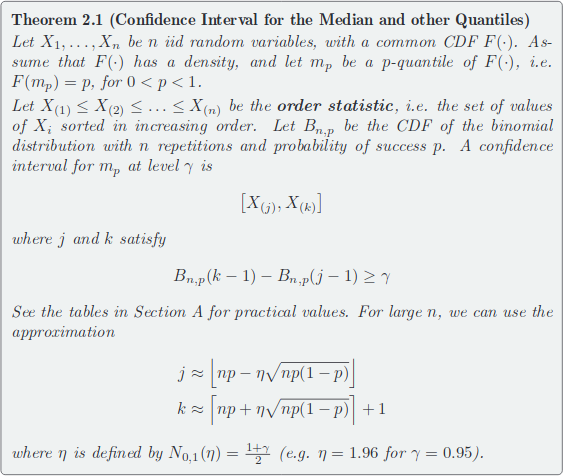
\includegraphics[width=0.7\linewidth]{illustrations/thereme-2-1-CI-median}
	\caption{Théorème 2.1 :  Confidence Interval for the Median and other Quantiles\cite{leboudec2010performance}}
	\label{fig:thereme-2-1-ci-median}
\end{figure}

\subsubsection{Le théorème 2.1 par l'exemple} \label{CI-theorem}

Les intervalles de confiance de la médiane des RTTs différentiels, appelée $\mu$, sont formulés par un calcul binomial et ils sont de type \textit{distribution free}. Ce type de distributions ne suivent pas une loi spécifique.
%De plus, ils ont utilisé le score de Wilson pour le calcul des deux bornes de l'intervalle.
Nous illustrons le calcul de l'intervalle de confiance de la médiane par un exemple.  Nous considérons  l'ensemble des données $X$ suivant : 
 \begin{center}
 $[7.92, 7.76, 8.16, 8.08, 7.68, 8.24, 8.32, 7.76, 8.72, 7.92]$
 \end{center}


Il s'agit d'un ensemble de $10$ éléments, nous commençons tout d'abord par ordonner ces $10$ éléments  par ordre croissant, nous obtenons l'ordre suivant :

\begin{table}[H]
	\centering
\begin{tabular}{lccccc!{\color{red}\vrule}ccccc}
\textbf{X}&	$ 7.68 $& $ 7.76 $& $ 7.76 $& $ 7.92 $& $ 7.92 $& $ 8.08  $& $ 8.16 $& $ 8.24 $& $ 8.32 $& $ 8.72 $\\ \hline
\textbf{Ordre}&	1&2&3&4&5&6&7&8&9&10\\
\end{tabular}
\end{table}

Nous avons $5$ valeurs inférieures ou égales à  $7.92$ et $5$ valeurs supérieures ou égales à $ 8.08 $. Ainsi l'intervalle [$ 7.92 $ , $ 8.08 $] est l'intervalle médian
et   $8$ ( $(7.92 + 8.08)/2 = 8 $) est la médiane.
%------------------------------------------
\begin{wrapfigure}{r}{.4\textwidth}
	\captionsetup{justification=centering}

	\resizebox{.4\textwidth}{!}{
		% Graphic for TeX using PGF
% Title: /home/hayat/RipeAtlasTraceroutesAnalysis/2019/Rapport/illustrations/medianeIllustra.dia
% Creator: Dia v0.97+git
% CreationDate: Sat Apr 27 13:08:32 2019
% For: hayat
% \usepackage{tikz}
% The following commands are not supported in PSTricks at present
% We define them conditionally, so when they are implemented,
% this pgf file will use them.
\ifx\du\undefined
  \newlength{\du}
\fi
\setlength{\du}{15\unitlength}
\begin{tikzpicture}[even odd rule]
\pgftransformxscale{1.000000}
\pgftransformyscale{-1.000000}
\definecolor{dialinecolor}{rgb}{0.000000, 0.000000, 0.000000}
\pgfsetstrokecolor{dialinecolor}
\pgfsetstrokeopacity{1.000000}
\definecolor{diafillcolor}{rgb}{1.000000, 1.000000, 1.000000}
\pgfsetfillcolor{diafillcolor}
\pgfsetfillopacity{1.000000}
\pgfsetlinewidth{0.100000\du}
\pgfsetdash{}{0pt}
\pgfsetbuttcap
{
\definecolor{diafillcolor}{rgb}{0.000000, 0.000000, 0.000000}
\pgfsetfillcolor{diafillcolor}
\pgfsetfillopacity{1.000000}
% was here!!!
\pgfsetarrowsend{stealth}
\definecolor{dialinecolor}{rgb}{0.000000, 0.000000, 0.000000}
\pgfsetstrokecolor{dialinecolor}
\pgfsetstrokeopacity{1.000000}
\draw (13.000000\du,15.950000\du)--(30.550000\du,15.900000\du);
}
\pgfsetlinewidth{0.100000\du}
\pgfsetdash{}{0pt}
\pgfsetbuttcap
{
\definecolor{diafillcolor}{rgb}{0.000000, 0.000000, 0.000000}
\pgfsetfillcolor{diafillcolor}
\pgfsetfillopacity{1.000000}
% was here!!!
\pgfsetarrowsend{stealth}
\definecolor{dialinecolor}{rgb}{0.000000, 0.000000, 0.000000}
\pgfsetstrokecolor{dialinecolor}
\pgfsetstrokeopacity{1.000000}
\draw (13.950000\du,16.800000\du)--(14.000000\du,6.400000\du);
}
\pgfsetlinewidth{0.100000\du}
\pgfsetdash{}{0pt}
\pgfsetmiterjoin
\pgfsetbuttcap
{
\definecolor{diafillcolor}{rgb}{0.000000, 0.000000, 0.000000}
\pgfsetfillcolor{diafillcolor}
\pgfsetfillopacity{1.000000}
% was here!!!
\definecolor{dialinecolor}{rgb}{0.000000, 0.000000, 0.000000}
\pgfsetstrokecolor{dialinecolor}
\pgfsetstrokeopacity{1.000000}
\pgfpathmoveto{\pgfpoint{14.400000\du}{14.950000\du}}
\pgfpathcurveto{\pgfpoint{17.404600\du}{14.950000\du}}{\pgfpoint{18.245400\du}{7.950000\du}}{\pgfpoint{21.250000\du}{7.950000\du}}
\pgfusepath{stroke}
}
\pgfsetlinewidth{0.100000\du}
\pgfsetdash{}{0pt}
\pgfsetmiterjoin
\pgfsetbuttcap
{
\definecolor{diafillcolor}{rgb}{0.000000, 0.000000, 0.000000}
\pgfsetfillcolor{diafillcolor}
\pgfsetfillopacity{1.000000}
% was here!!!
\definecolor{dialinecolor}{rgb}{0.000000, 0.000000, 0.000000}
\pgfsetstrokecolor{dialinecolor}
\pgfsetstrokeopacity{1.000000}
\pgfpathmoveto{\pgfpoint{21.300000\du}{7.950000\du}}
\pgfpathcurveto{\pgfpoint{24.719600\du}{7.950000\du}}{\pgfpoint{25.380400\du}{15.000000\du}}{\pgfpoint{28.800000\du}{15.000000\du}}
\pgfusepath{stroke}
}
\pgfsetlinewidth{0.100000\du}
\pgfsetdash{{\pgflinewidth}{0.200000\du}}{0cm}
\pgfsetbuttcap
{
\definecolor{diafillcolor}{rgb}{0.000000, 0.000000, 0.000000}
\pgfsetfillcolor{diafillcolor}
\pgfsetfillopacity{1.000000}
% was here!!!
\definecolor{dialinecolor}{rgb}{0.000000, 0.000000, 0.000000}
\pgfsetstrokecolor{dialinecolor}
\pgfsetstrokeopacity{1.000000}
\draw (21.200000\du,7.200000\du)--(21.200000\du,15.650000\du);
}
% setfont left to latex
\definecolor{dialinecolor}{rgb}{0.000000, 0.000000, 0.000000}
\pgfsetstrokecolor{dialinecolor}
\pgfsetstrokeopacity{1.000000}
\definecolor{diafillcolor}{rgb}{0.000000, 0.000000, 0.000000}
\pgfsetfillcolor{diafillcolor}
\pgfsetfillopacity{1.000000}
\node[anchor=base west,inner sep=0pt,outer sep=0pt,color=dialinecolor] at (18.595000\du,12.935000\du){50 \%};
% setfont left to latex
\definecolor{dialinecolor}{rgb}{0.000000, 0.000000, 0.000000}
\pgfsetstrokecolor{dialinecolor}
\pgfsetstrokeopacity{1.000000}
\definecolor{diafillcolor}{rgb}{0.000000, 0.000000, 0.000000}
\pgfsetfillcolor{diafillcolor}
\pgfsetfillopacity{1.000000}
\node[anchor=base west,inner sep=0pt,outer sep=0pt,color=dialinecolor] at (22.345000\du,13.000000\du){50 \%};
% setfont left to latex
\definecolor{dialinecolor}{rgb}{0.000000, 0.000000, 0.000000}
\pgfsetstrokecolor{dialinecolor}
\pgfsetstrokeopacity{1.000000}
\definecolor{diafillcolor}{rgb}{0.000000, 0.000000, 0.000000}
\pgfsetfillcolor{diafillcolor}
\pgfsetfillopacity{1.000000}
\node[anchor=base west,inner sep=0pt,outer sep=0pt,color=dialinecolor] at (20.945000\du,16.850000\du){\textmu};
\end{tikzpicture}


	}
			\caption{Illustration de la médiane}\label{fig:medianIllustration}
\end{wrapfigure} 
%------------------------------------------
 Par définition, la médiane d'un ensemble est la valeur qui permet de diviser cet ensemble en deux parties égales. Notre objectif est de quantifier  l'incertitude de la médiane calculée.
Soit \textmu, dans la Figure \ref{fig:medianIllustration},  la médiane d'une distribution donnée, c'est la valeur telle que $50\%$ des valeurs de la distribution sont au dessous de {\textmu}  et $50\%$ des valeurs de la distribution sont au dessus de  \textmu. Autrement dit, avec une probabilité de $50\%$ une valeur de \textit{X} est au dessous de {\textmu}  et avec une probabilité de $50\%$ une valeur de \textit{X} est au dessus de \textmu.

\begin{wrapfigure}{r}{.4\textwidth}
	\captionsetup{justification=centering}
	
	\resizebox{.4\textwidth}{!}{
		
		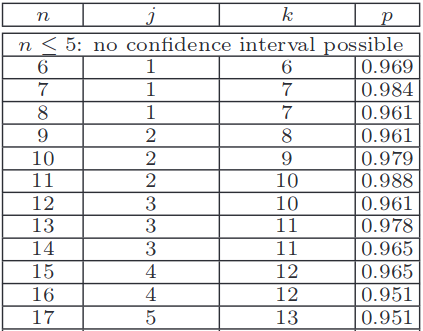
\includegraphics{illustrations/Table-CI-bis.png}
	}
	\caption{Table d'intervalles de confiance à $95\%$ \cite{leboudec2010performance}}\label{fig:tableCI}
\end{wrapfigure} 
 Il est clair que {\textmu} est une valeur unique. Ce que nous cherchons est d'approcher {\textmu}. Pour ce faire, nous allons appliquer le théorème 2.1 relatif au calcul de l'intervalle de confiance de la médiane. Ce théorème permet de calculer l'intervalle de confiance de la médiane d'un ensemble de données. Comme $n = 10 $, nous avons besoin d'une table comme celle  donnée dans la Figure \ref{fig:tableCI}. A partir de la taille de l'ensemble ($n$) et le niveau de confiance $\gamma$, il est possible de trouver la borne inférieure de l'intervalle de confiance ($X_{(j)}$) et la borne supérieure de l'intervalle de confiance ($X_{(k)}$) à une probabilité $p$. Cette table fournit l'intervalle de confiance à $95 \%$ de confiance pour tout $n \leq 70$. A partir de $n \geq 71$, nous utilisons les deux formules de $ j $ (\ref{align:formule-j}) et $ k $ (\ref{align:formule-k}).
 
Dans notre exemple,  $n = 10$, ainsi, à une probabilité $95\%$, $j = 2$ et $ k = 9$, revenons aux données ordonnées,  $ X_{(2)} = 7.76 $ et  $ X_{(9)} =8.32 $. Autrement dit, à $95\%$, il est sûr que la valeur réelle de la médiane de l'ensemble de données, utilisées pour l'exemple, se trouve dans l'intervalle $[7.76, 8.32]$.
 
\begin{align}
j&\approx \lfloor np - \eta  \sqrt{np(1-p)}\rfloor \label{align:formule-j}\\
k&\approx \lceil np + \eta  \sqrt{np(1-p)}\rceil + 1 \label{align:formule-k}
\end{align}

Prenons un exemple\footnote{Dans la table des intervalles de confiance, $p$ est le niveau de confiance, alors que ici, $p$ est la probabilité de succès.} où $n\geq 71$, soit p = 0.5 et $\eta$ = 1.96  pour  un intervalle de confiance à 95\%. Dans ce cas, 
$j \approx \lfloor 0.5n -  0.980\sqrt{n}\rfloor$ et $k\approx \lceil 0.5n + 0.980 \sqrt{n}\rceil + 1$.

Pour  $n = 100$ : $j = 40$ et $k = 61$, ainsi l'intervalle de confiance de la médiane est formé par $X_{(40)}$ et $X_{(61)}$.

Afin de montrer l'importance    de l'intervalle de confiance de la médiane dans l'élimination des valeurs aberrantes, nous donnons l'exemple suivant : 
 
\begin{table}[H]
	\centering
	\begin{tabular}{lccccc!{\color{red}\vrule}ccccc}
		\textbf{X}&	$ 7.68 $& $ 7.76 $& $ 7.76 $& $ 7.92 $& $ 8.08  $& $ 8.16 $& $ 8.24 $& $ 8.32 $& $ 8.72 $& $792$\\ \hline
		\textbf{Ordre}&	1&2&3&4&5&6&7&8&9&10\\
	\end{tabular}
\caption{Exemple 2 d'application du théorème 2.1}
\label{tab:outlierexample}
\end{table}

Le théorème $ 2.1 $ indique que l'intervalle de confiance de la médiane de l'ensemble de données dans la Table \ref{tab:outlierexample}  est formé par $ X_{(2)} $ et $X_{(9)}$, ce que donne $[7.76, 8.72]$ comme intervalle de confiance. L'intervalle de confiance obtenu pour cet ensemble de données est relativement différent de celui obtenu pour le premier ensemble de données. Toutefois, le deuxième intervalle de confiance est capable d'éliminer une valeur aberrante ($792$). 

\subsubsection{Méthode de score de  Wilson}
 Les auteurs ont choisi le score de Wilson pour trouver l'intervalle de confiance de la médiane,  car il fonctionne bien, même avec un  nombre réduit d'échantillons \cite{doi:10.1002/sim.2164}. Le score De Wilson est calculé avec la formule \ref{align:wilson-formula}, avec  $n$ est la taille de l'ensemble de données, $p$ est la probabilité de succès et $z$ est égale à $1.96$ pour un niveau de confiance égale à $95\%$.
\begin{align}
w&= \frac{1}{1 + \frac{1}{n}z^2} \left( p + \frac{1}{2n} z^2 \pm z \sqrt{\frac{1}{n}p(1-p)+ \frac{1}{4n^2}z^2} \right)\label{align:wilson-formula}
\end{align} 
En pratique, le score de Wilson  produit deux valeurs appelées $w_l$ et $w_u$ dont leur valeurs sont dans $[0, 1]$. En multipliant $w_l$ et $w_u$ par $n$, nous obtenons les indices de le borne inférieure $l = nw_l$  et supérieure $u = nw_u$ de l'intervalle de confiance de la médiane. Nous précisons qu'en pratique, seule la partie entière de $l$ et $u$ qui indique l'indice. 
 De la même manière que la méthode décrite dans la section \ref{CI-theorem}, nous ordonnons les $n$ données et nous construisons l'intervalle $[X_{(l)}, X_{(u)}]$.


En se basant uniquement sur l'ordre statistique, le score de Wilson produit des intervalles de confiance asymétriques dans le cas de distributions asymétriques, ce qui est le cas  des distributions des RTTs d'après l'étude \cite{DBLP:conf/infocom/FontugneMF15}. En outre, cette technique de calcul, basée uniquement sur l'ordre statistique de la variable permet d'éliminer les valeurs aberrantes indésirables.

Pour résumer, tout lien et pour chaque période, il est caractérisé par un ensemble de RTTs différentiels. Sur base de cet ensemble, les auteurs ont pu  caractériser ce lien par  la médiane  des RTTs différentiels.  De plus, en se basant encore sur cet ensemble, ils ont calculé l'intervalle de confiance de cette médiane. De la même manière, ils ont calculé une référence reprenant la médiane des RTTs différentiels et son intervalle de confiance. Cette référence prend en considération les observations des périodes précédentes.  

\subsection{Calcul de la référence} \label{reference-lissage}
L'état référence d'un lien représente le délai habituel d'un lien avec son intervalle de confiance habituel. Cette référence est utilisée pour détecter les délais anormaux. Précisément, cette référence est conservée  et  est mise à jour tout au long de l'analyse. C'est avec cette référence que l'état courant du lien est comparé. 
 %Les auteurs ont proposé  l'approche  suivante, c'est comparer les deux intervalles de référence courant et référence. 

Présentons  brièvement  les séries chronologiques et leurs caractéristiques \cite{elementdestatistiques}.   
\begin{tcolorbox}[before upper={\parindent15pt}]
	Une \textit{série chronologique} est une série d'observations d'une variable réalisées à des dates successives notées $d_1$, $d_2$, ..., $d_n$. On distingue deux types de variables :
	
	\textit{variable  d'intensité} : les variables d'intensité, encore appelées \textbf{niveaux}, prennent leurs valeurs en des instants précis. Il en est de la température relevée dans un local tous les matins à $8$ heures, etc.
	
	\textit{variable de débit} : les variables de débit, encore appelées \textbf{flux}, concernent des intervalles de temps. C'est le cas, par exemple, de la quantité d'électricité consommée chaque jour par un ménage, etc.
	
	Si, dans le premier cas, les dates d'observation correspondent effectivement aux instants de mesure, le second cas, il est fréquent d'utiliser une notation unique; d'affecter la valeur observée pour une période déterminée au début de cette dernière, au centre ou à autre.
	
	L'étude d'une série chronologique concerne généralement trois objectifs : la description du phénomène étudié, son lissage et la détermination de prévisions.
\end{tcolorbox}

Dans notre cas, ce sont des périodes personnalisables, généralement une période d'une heure et les RTTs différentiels calculés durant, par exemple, une heure sont affectés au début de la période.

Etant donné que la médiane des RTTs différentiels est distribuée normalement,  la valeur prévue de la médiane est obtenue simplement en calculant la moyenne arithmétique des médianes observées précédemment, c'est qu'on appelle \textit{la moyenne mobile simple}. \textit{Cette manière d'agir ne se conçoit empiriquement que si le phénomène est stable\footnote{Prévision par moyenne mobile simple unilatérale (6.10.3)\cite{elementdestatistiques}.}}.
Etant donné que les anomalies peuvent altérer les valeurs moyennes et les rendre non pertinentes en tant que références, les auteurs ont utilisé    une prévision par lissage exponentiel 
plutôt qu'une prévision par moyenne mobile simple  en vue d'estimer la médiane des RTTs différentiels de référence tout en réduisant l'effet des anomalies sur cette médiane.
Si  la moyenne mobile simple  prend en compte les valeurs passées avec le même coefficient de pondération,  la prévision par lissage exponentiel peut supposer que plus une observation est ancienne, moins elle intervient dans la détermination de la prévision. 

Pour calculer la  valeur de la médiane des RTTs différentiels de référence $ \overline{m}_{t}$   courant la période $ t $ et pour le lien $l$, soit:

\begin{align}
	 \overline{m}_{t}& =  \alpha {m}_{t} + (1-  \alpha) \overline{m}_{t-1} \label{smoothe-formula}
\end{align} 

$m_t$ est la médiane des RTTs différentiels observée pour $l$ durant la période $t$. 

$ \overline{m}_{t-1}$  est la médiane des  RTTs différentiels  de référence durant la période $ t-1 $.  
$\alpha$ est un paramètre réel dans $[0,1]$, ce paramètre contrôle l'importance des nouvelles observations par rapport aux celles anciennes. Dans le cas de la présente étude, $\alpha$ est préféré d'être petit, précisément, $ \alpha = 0.01$.

Par ailleurs, l'utilisation de la formule \ref{smoothe-formula} pour la prévision de la médiane de référence nécessite de définir la valeur de la médiane initiale $ {m}_{1}$. Il existe plusieurs possibilités pour calculer $ {m}_{1}$, par exemple, il est possible de la définir comme étant la moyenne de deux, trois ou plusieurs premières observations. Dans leur implémentation, les auteurs ont choisi $\overline{m}_{1}$ comme étant la médiane de toutes les médianes des RTTs différentiels de $minSeen$  périodes, où $minSeen$ est un entier. Pour le reste des prévisions de la médiane de référence, on implique la médiane de référence précédente et  la médiane courante.

la référence d'un lien ne se limite pas seulement sur la médiane des RTTs différentiels mais en plus de la médiane,  on calcule  l'intervalle de confiance habituel de cette médiane. Les bornes de ce dernier sont calculées de la même manière que la médiane. Autrement dit, nous effectuons au fur et au mesure la prévision par lissage exponentiel de la borne inférieure de l'intervalle de confiance (respectivement borne supérieure). 

A ce stade, nous pouvons décrire un lien, durant une période donnée, par la médiane des RTTs différentiels et son intervalle de confiance. Ces même éléments illustre à la fois l'état courant du lien ainsi que son état référence. Sur base de ces état, on peut déclencher la détection des changements dans les délais de ce lien.

%Soient $d_i$, $d_j$, $d_k$, $d_l$, $d_m$ et $d_n$ des périodes quelconques  de l'analyse, et
Prenons un exemple où nous calculons la borne inférieure de l'intervalle de confiance de référence. 
Soient \textit{curCiLow} et \textit{refCiLow} la borne inférieure de l'intervalle de confiance de médiane courante et la borne inférieure de l'intervalle de confiance de la médiane référence.
Soit  $minSeen = 4$ le nombre d'observations assurant la représentativité de la référence. Soit $d_i$ la période courante de l'analyse et $d_1, d_2, ..., d_t$ les périodes de l'analyse. Nous distinguons trois cas :
\begin{itemize}
	\item  $d_i< d_{minSeen}$ : l'état référence est égal à l'état courant.
	\item  $d_i = d_{minSeen}$ : calcul de la référence pour la première fois en calculant la médiane de toutes les observations précédentes.
	\item  $d_i >d_{minSeen}$ : calcul de la référence en impliquant l'état courant et la référence précédente en appliquant l'équation \ref{smoothe-formula}.
\end{itemize}

Ces trois cas sont illustrés dans les  Tables \ref{result-3-cas}, ces derniers reprennent les résultats de l'analyse d'un nombre de traceroutes\footnote{\url{https://github.com/hayatbellafkih/SparkSalacaTraceroutesAnalysis/blob/master/rttDelaysSparkScala/src/main/resources/test/result_modified.json}, consultée  le $23/04/2019$. }.

\begin{table}[h]
	\captionsetup{justification= centering}
	
	\footnotesize{

	\caption{Exemple de calcul et mise à jour de la borne inférieure de l'intervalle  de confiance référence de la médiane }
\label{result-3-cas}
	\begin{minipage}{.3\linewidth}
		
		\caption*{$d_i< d_{minSeen}$}
		\centering
		\begin{tabular}{|c|c|c|}
			\hline
			\textbf{$\mathbf{d_i}$} & \textbf{\textit{curCiLow}} &\textbf{\textit{refCiLow}} \\\hline
			$d_1$ &-3.197& -3.197\\\hline
			$d_2$ & -2.968&-2.968 \\\hline
			$d_3$ & -3.201& -3.201 \\\hline
		\end{tabular}
	
	\end{minipage}%
	\begin{minipage}{.3\linewidth}
	\caption*{ $d_i = d_{minSeen}$}
	\centering
		\begin{tabular}{|c|c|c|}
	\hline
			\textbf{$\mathbf{d_i}$} & \textbf{\textit{curCiLow}} &\textbf{\textit{refCiLow}} \\\hline
	$d_1$ &-3.197&-3.197\\\hline
	$d_2$ & -2.968&-3.197 \\\hline
	$d_3$ & -3.201& -3.197 \\\hline
	$d_4$ &-998.029& -3.197\\\hline
\end{tabular}
\end{minipage}%
	\begin{minipage}{.4\linewidth}
		\centering
		\caption*{$d_i >d_{minSeen}$}
		\begin{tabular}{|c|c|c|}
	\hline
			\textbf{$\mathbf{d_i}$} & \textbf{\textit{curCiLow}} &\textbf{\textit{refCiLow}} \\\hline
	$ d_1$ &-3.197&-3.197\\\hline
	$d_2$ & -2.968&-3.197 \\\hline
	$d_3$ & -3.201& -3.197 \\\hline
	$d_4$ &-998.029& -3.197\\\hline
	$d_5$ &-1098.029& -14.14532\\\hline
	$d_6$ &-3.029& -14.0341568\\\hline
\end{tabular}
	\end{minipage} 
}

\end{table}


\subsubsection{Détection des anomalies}
Afin d'identifier un changement dans le délai d'un lien, il suffit de comparer l'intervalle de confiance courant avec l'intervalle de 
confiance de référence. Cette comparaison ne se déclenche que si la référence de ce lien est assez représentable, autrement dit, le nombre d'observations est atteint pour calculer $\overline{m}_{1}$. Ce nombre est personnalisable et par défaut il est configuré sur $ 24 $. Si par exemple la durée d'une période est 1 heure, il faut avoir une journée d'observation pour construire la première référence du lien en question. Une fois la référence est  assez représentable, dorénavant,  elle est mise à jour en utilisant  le lissage exponentiel décrit dans la section \ref{reference-lissage}.
\begin{wrapfigure}{r}{.4\textwidth}
	\captionsetup{justification=centering}
	
	\resizebox{.4\textwidth}{!}{
		% Graphic for TeX using PGF
% Title: /home/hayat/RipeAtlasTraceroutesAnalysis/2019/Rapport/illustrations/explainCis
% Creator: Dia v0.97+git
% CreationDate: Tue Apr 30 10:45:36 2019
% For: hayat
% \usepackage{tikz}
% The following commands are not supported in PSTricks at present
% We define them conditionally, so when they are implemented,
% this pgf file will use them.
\ifx\du\undefined
  \newlength{\du}
\fi
\setlength{\du}{15\unitlength}
\begin{tikzpicture}[even odd rule]
\pgftransformxscale{1.000000}
\pgftransformyscale{-1.000000}
\definecolor{dialinecolor}{rgb}{0.000000, 0.000000, 0.000000}
\pgfsetstrokecolor{dialinecolor}
\pgfsetstrokeopacity{1.000000}
\definecolor{diafillcolor}{rgb}{1.000000, 1.000000, 1.000000}
\pgfsetfillcolor{diafillcolor}
\pgfsetfillopacity{1.000000}
\pgfsetlinewidth{0.100000\du}
\pgfsetdash{}{0pt}
\pgfsetbuttcap
{
\definecolor{diafillcolor}{rgb}{0.000000, 0.000000, 0.000000}
\pgfsetfillcolor{diafillcolor}
\pgfsetfillopacity{1.000000}
% was here!!!
}
\definecolor{dialinecolor}{rgb}{0.000000, 0.000000, 0.000000}
\pgfsetstrokecolor{dialinecolor}
\pgfsetstrokeopacity{1.000000}
\draw (11.337256\du,5.581598\du)--(11.354934\du,10.884899\du);
\pgfsetlinewidth{0.100000\du}
\pgfsetdash{}{0pt}
\pgfsetmiterjoin
\pgfsetbuttcap
\definecolor{diafillcolor}{rgb}{0.000000, 0.000000, 0.000000}
\pgfsetfillcolor{diafillcolor}
\pgfsetfillopacity{1.000000}
\definecolor{dialinecolor}{rgb}{0.000000, 0.000000, 0.000000}
\pgfsetstrokecolor{dialinecolor}
\pgfsetstrokeopacity{1.000000}
\pgfpathmoveto{\pgfpoint{11.337256\du}{5.581598\du}}
\pgfpathcurveto{\pgfpoint{11.462256\du}{5.581181\du}}{\pgfpoint{11.587671\du}{5.705764\du}}{\pgfpoint{11.588088\du}{5.830763\du}}
\pgfpathcurveto{\pgfpoint{11.588505\du}{5.955763\du}}{\pgfpoint{11.463922\du}{6.081179\du}}{\pgfpoint{11.338923\du}{6.081595\du}}
\pgfpathcurveto{\pgfpoint{11.213924\du}{6.082012\du}}{\pgfpoint{11.088508\du}{5.957429\du}}{\pgfpoint{11.088091\du}{5.832430\du}}
\pgfpathcurveto{\pgfpoint{11.087674\du}{5.707431\du}}{\pgfpoint{11.212257\du}{5.582015\du}}{\pgfpoint{11.337256\du}{5.581598\du}}
\pgfpathclose
\pgfusepath{fill,stroke}
\pgfsetlinewidth{0.100000\du}
\pgfsetdash{}{0pt}
\pgfsetmiterjoin
\pgfsetbuttcap
\definecolor{diafillcolor}{rgb}{0.000000, 0.000000, 0.000000}
\pgfsetfillcolor{diafillcolor}
\pgfsetfillopacity{1.000000}
\definecolor{dialinecolor}{rgb}{0.000000, 0.000000, 0.000000}
\pgfsetstrokecolor{dialinecolor}
\pgfsetstrokeopacity{1.000000}
\pgfpathmoveto{\pgfpoint{11.354934\du}{10.884899\du}}
\pgfpathcurveto{\pgfpoint{11.229935\du}{10.885316\du}}{\pgfpoint{11.104519\du}{10.760733\du}}{\pgfpoint{11.104102\du}{10.635734\du}}
\pgfpathcurveto{\pgfpoint{11.103685\du}{10.510734\du}}{\pgfpoint{11.228268\du}{10.385318\du}}{\pgfpoint{11.353267\du}{10.384902\du}}
\pgfpathcurveto{\pgfpoint{11.478267\du}{10.384485\du}}{\pgfpoint{11.603683\du}{10.509068\du}}{\pgfpoint{11.604099\du}{10.634067\du}}
\pgfpathcurveto{\pgfpoint{11.604516\du}{10.759066\du}}{\pgfpoint{11.479933\du}{10.884482\du}}{\pgfpoint{11.354934\du}{10.884899\du}}
\pgfpathclose
\pgfusepath{fill,stroke}
% setfont left to latex
\definecolor{dialinecolor}{rgb}{0.000000, 0.000000, 0.000000}
\pgfsetstrokecolor{dialinecolor}
\pgfsetstrokeopacity{1.000000}
\definecolor{diafillcolor}{rgb}{0.000000, 0.000000, 0.000000}
\pgfsetfillcolor{diafillcolor}
\pgfsetfillopacity{1.000000}
\node[anchor=base west,inner sep=0pt,outer sep=0pt,color=dialinecolor] at (11.100944\du,8.615472\du){-};
\pgfsetlinewidth{0.100000\du}
\pgfsetdash{}{0pt}
\pgfsetbuttcap
{
\definecolor{diafillcolor}{rgb}{0.000000, 0.000000, 0.000000}
\pgfsetfillcolor{diafillcolor}
\pgfsetfillopacity{1.000000}
% was here!!!
}
\definecolor{dialinecolor}{rgb}{0.000000, 0.000000, 0.000000}
\pgfsetstrokecolor{dialinecolor}
\pgfsetstrokeopacity{1.000000}
\draw (13.281660\du,6.080057\du)--(13.276752\du,10.374707\du);
\pgfsetlinewidth{0.100000\du}
\pgfsetdash{}{0pt}
\pgfsetmiterjoin
\pgfsetbuttcap
\definecolor{diafillcolor}{rgb}{1.000000, 1.000000, 1.000000}
\pgfsetfillcolor{diafillcolor}
\pgfsetfillopacity{1.000000}
\definecolor{dialinecolor}{rgb}{0.000000, 0.000000, 0.000000}
\pgfsetstrokecolor{dialinecolor}
\pgfsetstrokeopacity{1.000000}
\pgfpathmoveto{\pgfpoint{13.282231\du}{5.580057\du}}
\pgfpathcurveto{\pgfpoint{13.407231\du}{5.580200\du}}{\pgfpoint{13.532088\du}{5.705343\du}}{\pgfpoint{13.531945\du}{5.830343\du}}
\pgfpathcurveto{\pgfpoint{13.531802\du}{5.955343\du}}{\pgfpoint{13.406660\du}{6.080200\du}}{\pgfpoint{13.281660\du}{6.080057\du}}
\pgfpathcurveto{\pgfpoint{13.156660\du}{6.079914\du}}{\pgfpoint{13.031803\du}{5.954771\du}}{\pgfpoint{13.031946\du}{5.829771\du}}
\pgfpathcurveto{\pgfpoint{13.032088\du}{5.704771\du}}{\pgfpoint{13.157231\du}{5.579914\du}}{\pgfpoint{13.282231\du}{5.580057\du}}
\pgfpathclose
\pgfusepath{fill,stroke}
\pgfsetlinewidth{0.100000\du}
\pgfsetdash{}{0pt}
\pgfsetmiterjoin
\pgfsetbuttcap
\definecolor{diafillcolor}{rgb}{1.000000, 1.000000, 1.000000}
\pgfsetfillcolor{diafillcolor}
\pgfsetfillopacity{1.000000}
\definecolor{dialinecolor}{rgb}{0.000000, 0.000000, 0.000000}
\pgfsetstrokecolor{dialinecolor}
\pgfsetstrokeopacity{1.000000}
\pgfpathmoveto{\pgfpoint{13.276180\du}{10.874707\du}}
\pgfpathcurveto{\pgfpoint{13.151180\du}{10.874564\du}}{\pgfpoint{13.026323\du}{10.749421\du}}{\pgfpoint{13.026466\du}{10.624421\du}}
\pgfpathcurveto{\pgfpoint{13.026609\du}{10.499421\du}}{\pgfpoint{13.151752\du}{10.374564\du}}{\pgfpoint{13.276752\du}{10.374707\du}}
\pgfpathcurveto{\pgfpoint{13.401751\du}{10.374850\du}}{\pgfpoint{13.526609\du}{10.499993\du}}{\pgfpoint{13.526466\du}{10.624993\du}}
\pgfpathcurveto{\pgfpoint{13.526323\du}{10.749993\du}}{\pgfpoint{13.401180\du}{10.874850\du}}{\pgfpoint{13.276180\du}{10.874707\du}}
\pgfpathclose
\pgfusepath{fill,stroke}
% setfont left to latex
\definecolor{dialinecolor}{rgb}{0.000000, 0.000000, 0.000000}
\pgfsetstrokecolor{dialinecolor}
\pgfsetstrokeopacity{1.000000}
\definecolor{diafillcolor}{rgb}{0.000000, 0.000000, 0.000000}
\pgfsetfillcolor{diafillcolor}
\pgfsetfillopacity{1.000000}
\node[anchor=base west,inner sep=0pt,outer sep=0pt,color=dialinecolor] at (13.012306\du,8.716238\du){*};
% setfont left to latex
\definecolor{dialinecolor}{rgb}{0.000000, 0.000000, 0.000000}
\pgfsetstrokecolor{dialinecolor}
\pgfsetstrokeopacity{1.000000}
\definecolor{diafillcolor}{rgb}{0.000000, 0.000000, 0.000000}
\pgfsetfillcolor{diafillcolor}
\pgfsetfillopacity{1.000000}
\node[anchor=base west,inner sep=0pt,outer sep=0pt,color=dialinecolor] at (14.943501\du,6.005862\du){referenceCiLow};
% setfont left to latex
\definecolor{dialinecolor}{rgb}{0.000000, 0.000000, 0.000000}
\pgfsetstrokecolor{dialinecolor}
\pgfsetstrokeopacity{1.000000}
\definecolor{diafillcolor}{rgb}{0.000000, 0.000000, 0.000000}
\pgfsetfillcolor{diafillcolor}
\pgfsetfillopacity{1.000000}
\node[anchor=base west,inner sep=0pt,outer sep=0pt,color=dialinecolor] at (14.977088\du,10.910678\du){referenceCiHight};
\pgfsetlinewidth{0.100000\du}
\pgfsetdash{}{0pt}
\pgfsetbuttcap
{
\definecolor{diafillcolor}{rgb}{0.000000, 0.000000, 0.000000}
\pgfsetfillcolor{diafillcolor}
\pgfsetfillopacity{1.000000}
% was here!!!
\pgfsetarrowsend{to}
\definecolor{dialinecolor}{rgb}{0.000000, 0.000000, 0.000000}
\pgfsetstrokecolor{dialinecolor}
\pgfsetstrokeopacity{1.000000}
\draw (14.749046\du,5.776052\du)--(13.723742\du,5.776052\du);
}
\pgfsetlinewidth{0.100000\du}
\pgfsetdash{}{0pt}
\pgfsetbuttcap
{
\definecolor{diafillcolor}{rgb}{0.000000, 0.000000, 0.000000}
\pgfsetfillcolor{diafillcolor}
\pgfsetfillopacity{1.000000}
% was here!!!
\pgfsetarrowsend{to}
\definecolor{dialinecolor}{rgb}{0.000000, 0.000000, 0.000000}
\pgfsetstrokecolor{dialinecolor}
\pgfsetstrokeopacity{1.000000}
\draw (14.885667\du,10.752646\du)--(13.860362\du,10.752646\du);
}
% setfont left to latex
\definecolor{dialinecolor}{rgb}{0.000000, 0.000000, 0.000000}
\pgfsetstrokecolor{dialinecolor}
\pgfsetstrokeopacity{1.000000}
\definecolor{diafillcolor}{rgb}{0.000000, 0.000000, 0.000000}
\pgfsetfillcolor{diafillcolor}
\pgfsetfillopacity{1.000000}
\node[anchor=base west,inner sep=0pt,outer sep=0pt,color=dialinecolor] at (14.959411\du,8.365094\du){referenceMedian};
\pgfsetlinewidth{0.100000\du}
\pgfsetdash{}{0pt}
\pgfsetbuttcap
{
\definecolor{diafillcolor}{rgb}{0.000000, 0.000000, 0.000000}
\pgfsetfillcolor{diafillcolor}
\pgfsetfillopacity{1.000000}
% was here!!!
\pgfsetarrowsend{to}
\definecolor{dialinecolor}{rgb}{0.000000, 0.000000, 0.000000}
\pgfsetstrokecolor{dialinecolor}
\pgfsetstrokeopacity{1.000000}
\draw (14.832634\du,8.189384\du)--(13.807329\du,8.189384\du);
}
% setfont left to latex
\definecolor{dialinecolor}{rgb}{0.000000, 0.000000, 0.000000}
\pgfsetstrokecolor{dialinecolor}
\pgfsetstrokeopacity{1.000000}
\definecolor{diafillcolor}{rgb}{0.000000, 0.000000, 0.000000}
\pgfsetfillcolor{diafillcolor}
\pgfsetfillopacity{1.000000}
\node[anchor=base west,inner sep=0pt,outer sep=0pt,color=dialinecolor] at (4.968494\du,6.031641\du){currentCiLow};
% setfont left to latex
\definecolor{dialinecolor}{rgb}{0.000000, 0.000000, 0.000000}
\pgfsetstrokecolor{dialinecolor}
\pgfsetstrokeopacity{1.000000}
\definecolor{diafillcolor}{rgb}{0.000000, 0.000000, 0.000000}
\pgfsetfillcolor{diafillcolor}
\pgfsetfillopacity{1.000000}
\node[anchor=base west,inner sep=0pt,outer sep=0pt,color=dialinecolor] at (4.913694\du,10.706647\du){currentCiHight};
\pgfsetlinewidth{0.100000\du}
\pgfsetdash{}{0pt}
\pgfsetbuttcap
{
\definecolor{diafillcolor}{rgb}{0.000000, 0.000000, 0.000000}
\pgfsetfillcolor{diafillcolor}
\pgfsetfillopacity{1.000000}
% was here!!!
\pgfsetarrowsstart{to}
\definecolor{dialinecolor}{rgb}{0.000000, 0.000000, 0.000000}
\pgfsetstrokecolor{dialinecolor}
\pgfsetstrokeopacity{1.000000}
\draw (10.797325\du,10.637003\du)--(9.772020\du,10.637003\du);
}
% setfont left to latex
\definecolor{dialinecolor}{rgb}{0.000000, 0.000000, 0.000000}
\pgfsetstrokecolor{dialinecolor}
\pgfsetstrokeopacity{1.000000}
\definecolor{diafillcolor}{rgb}{0.000000, 0.000000, 0.000000}
\pgfsetfillcolor{diafillcolor}
\pgfsetfillopacity{1.000000}
\node[anchor=base west,inner sep=0pt,outer sep=0pt,color=dialinecolor] at (5.037437\du,8.355517\du){currentMedian};
\pgfsetlinewidth{0.100000\du}
\pgfsetdash{}{0pt}
\pgfsetbuttcap
{
\definecolor{diafillcolor}{rgb}{0.000000, 0.000000, 0.000000}
\pgfsetfillcolor{diafillcolor}
\pgfsetfillopacity{1.000000}
% was here!!!
\pgfsetarrowsstart{to}
\definecolor{dialinecolor}{rgb}{0.000000, 0.000000, 0.000000}
\pgfsetstrokecolor{dialinecolor}
\pgfsetstrokeopacity{1.000000}
\draw (10.961224\du,8.207061\du)--(9.935920\du,8.207061\du);
}
\pgfsetlinewidth{0.100000\du}
\pgfsetdash{}{0pt}
\pgfsetbuttcap
{
\definecolor{diafillcolor}{rgb}{0.000000, 0.000000, 0.000000}
\pgfsetfillcolor{diafillcolor}
\pgfsetfillopacity{1.000000}
% was here!!!
\pgfsetarrowsstart{to}
\definecolor{dialinecolor}{rgb}{0.000000, 0.000000, 0.000000}
\pgfsetstrokecolor{dialinecolor}
\pgfsetstrokeopacity{1.000000}
\draw (10.977134\du,5.887751\du)--(9.951829\du,5.887751\du);
}
\end{tikzpicture}

	}
	\caption{Nomination utilisée}
	\label{fig:explainCis}
\end{wrapfigure}

 
  Soit \textit{currentCiLow}, \textit{currentCiHight}, \textit{currentMedian}, \textit{referenceCiLow}, \textit{referenceCiHight}, \textit{referenceMedian} dénote respectivement la borne inférieure de l'intervalle de confiance de médiane courante, la borne supérieure de l'intervalle de confiance de la médiane courante, la médiane des RTTs différentiels courante, la borne inférieure de l'intervalle de confiance de la médiane de référence, la borne supérieure de l'intervalle de confiance de la médiane de référence, la médiane des RTTs différentiels de référence. La Figure 	\ref{fig:explainCis} illustre la nomination utilisée dans la Figure \ref{fig:anomalies}.
 
  Dans le travail de référence, une anomalie est détectée si les conditions \ref{align:condition-1} et \ref{align:condition-2} sont vraies. La première condition évalue le chevauchement entre les deux intervalles de confiance. Or, la deuxième condition assure que seulement la  différence entre la médiane des RTTs différentiels courante et celle de référence dépassant $1 ms$ qui est prise en compte.
\begin{align}
(currentCiLow > referenceCiHight OU  currentCiHight <  referenceCiLow) \label{align:condition-1}
\end{align}
\begin{align}
(abs(currentMedian -- referenceMedian) > 1 ) \label{align:condition-2}
\end{align}
  %Nous illustrons la comparaison des intervalles de confiance dans la Figure \ref{fig:anomalies}.
La Figure \ref{fig:anomalies} illustre les différents cas possibles de positionnement des deux intervalles de confiance. Nous précisons que,  dans les Figures	\ref{fig:explainCis} et \ref{fig:anomalies},  la longueur des intervalles de confiance ainsi que le positionnement de la médiane n'est pas exacte, ils sont donnés pour l'illustration de la comparaison. Nous supposons que la condition \ref{align:condition-2} est vraie et les différents cas possibles sont donnés dans la Figure 	\ref{fig:anomalies}.

\begin{figure}[H]
	\centering
	\captionsetup{justification=centering}
	\resizebox{\textwidth}{!}{
		% Graphic for TeX using PGF
% Title: /home/hayat/RipeAtlasTraceroutesAnalysis/2019/Rapport/illustrations/casesAnomalies.dia
% Creator: Dia v0.97+git
% CreationDate: Tue Apr 30 01:04:07 2019
% For: hayat
% \usepackage{tikz}
% The following commands are not supported in PSTricks at present
% We define them conditionally, so when they are implemented,
% this pgf file will use them.
\ifx\du\undefined
  \newlength{\du}
\fi
\setlength{\du}{15\unitlength}
\begin{tikzpicture}[even odd rule]
\pgftransformxscale{1.000000}
\pgftransformyscale{-1.000000}
\definecolor{dialinecolor}{rgb}{0.000000, 0.000000, 0.000000}
\pgfsetstrokecolor{dialinecolor}
\pgfsetstrokeopacity{1.000000}
\definecolor{diafillcolor}{rgb}{1.000000, 1.000000, 1.000000}
\pgfsetfillcolor{diafillcolor}
\pgfsetfillopacity{1.000000}
\pgfsetlinewidth{0.100000\du}
\pgfsetdash{}{0pt}
\pgfsetbuttcap
{
\definecolor{diafillcolor}{rgb}{0.000000, 0.000000, 0.000000}
\pgfsetfillcolor{diafillcolor}
\pgfsetfillopacity{1.000000}
% was here!!!
\pgfsetarrowsend{stealth}
\definecolor{dialinecolor}{rgb}{0.000000, 0.000000, 0.000000}
\pgfsetstrokecolor{dialinecolor}
\pgfsetstrokeopacity{1.000000}
\draw (5.463816\du,9.994870\du)--(56.365537\du,10.059352\du);
}
\pgfsetlinewidth{0.100000\du}
\pgfsetdash{}{0pt}
\pgfsetbuttcap
{
\definecolor{diafillcolor}{rgb}{0.000000, 0.000000, 0.000000}
\pgfsetfillcolor{diafillcolor}
\pgfsetfillopacity{1.000000}
% was here!!!
\pgfsetarrowsend{stealth}
\definecolor{dialinecolor}{rgb}{0.000000, 0.000000, 0.000000}
\pgfsetstrokecolor{dialinecolor}
\pgfsetstrokeopacity{1.000000}
\draw (8.950025\du,10.850000\du)--(8.977679\du,-3.524568\du);
}
\pgfsetlinewidth{0.100000\du}
\pgfsetdash{}{0pt}
\pgfsetbuttcap
{
\definecolor{diafillcolor}{rgb}{0.000000, 0.000000, 0.000000}
\pgfsetfillcolor{diafillcolor}
\pgfsetfillopacity{1.000000}
% was here!!!
}
\definecolor{dialinecolor}{rgb}{0.000000, 0.000000, 0.000000}
\pgfsetstrokecolor{dialinecolor}
\pgfsetstrokeopacity{1.000000}
\draw (17.091618\du,5.650000\du)--(17.091726\du,9.300000\du);
\pgfsetlinewidth{0.100000\du}
\pgfsetdash{}{0pt}
\pgfsetmiterjoin
\pgfsetbuttcap
\definecolor{diafillcolor}{rgb}{0.000000, 0.000000, 0.000000}
\pgfsetfillcolor{diafillcolor}
\pgfsetfillopacity{1.000000}
\definecolor{dialinecolor}{rgb}{0.000000, 0.000000, 0.000000}
\pgfsetstrokecolor{dialinecolor}
\pgfsetstrokeopacity{1.000000}
\pgfpathmoveto{\pgfpoint{17.091618\du}{5.650000\du}}
\pgfpathcurveto{\pgfpoint{17.216618\du}{5.649996\du}}{\pgfpoint{17.341622\du}{5.774993\du}}{\pgfpoint{17.341625\du}{5.899993\du}}
\pgfpathcurveto{\pgfpoint{17.341629\du}{6.024993\du}}{\pgfpoint{17.216633\du}{6.149996\du}}{\pgfpoint{17.091633\du}{6.150000\du}}
\pgfpathcurveto{\pgfpoint{16.966633\du}{6.150004\du}}{\pgfpoint{16.841629\du}{6.025007\du}}{\pgfpoint{16.841625\du}{5.900007\du}}
\pgfpathcurveto{\pgfpoint{16.841622\du}{5.775007\du}}{\pgfpoint{16.966618\du}{5.650004\du}}{\pgfpoint{17.091618\du}{5.650000\du}}
\pgfpathclose
\pgfusepath{fill,stroke}
\pgfsetlinewidth{0.100000\du}
\pgfsetdash{}{0pt}
\pgfsetmiterjoin
\pgfsetbuttcap
\definecolor{diafillcolor}{rgb}{0.000000, 0.000000, 0.000000}
\pgfsetfillcolor{diafillcolor}
\pgfsetfillopacity{1.000000}
\definecolor{dialinecolor}{rgb}{0.000000, 0.000000, 0.000000}
\pgfsetstrokecolor{dialinecolor}
\pgfsetstrokeopacity{1.000000}
\pgfpathmoveto{\pgfpoint{17.091726\du}{9.300000\du}}
\pgfpathcurveto{\pgfpoint{16.966726\du}{9.300004\du}}{\pgfpoint{16.841723\du}{9.175007\du}}{\pgfpoint{16.841719\du}{9.050007\du}}
\pgfpathcurveto{\pgfpoint{16.841715\du}{8.925007\du}}{\pgfpoint{16.966712\du}{8.800004\du}}{\pgfpoint{17.091712\du}{8.800000\du}}
\pgfpathcurveto{\pgfpoint{17.216712\du}{8.799996\du}}{\pgfpoint{17.341715\du}{8.924993\du}}{\pgfpoint{17.341719\du}{9.049993\du}}
\pgfpathcurveto{\pgfpoint{17.341723\du}{9.174993\du}}{\pgfpoint{17.216726\du}{9.299996\du}}{\pgfpoint{17.091726\du}{9.300000\du}}
\pgfpathclose
\pgfusepath{fill,stroke}
\pgfsetlinewidth{0.100000\du}
\pgfsetdash{}{0pt}
\pgfsetbuttcap
{
\definecolor{diafillcolor}{rgb}{0.000000, 0.000000, 0.000000}
\pgfsetfillcolor{diafillcolor}
\pgfsetfillopacity{1.000000}
% was here!!!
}
\definecolor{dialinecolor}{rgb}{0.000000, 0.000000, 0.000000}
\pgfsetstrokecolor{dialinecolor}
\pgfsetstrokeopacity{1.000000}
\draw (19.099686\du,0.525845\du)--(19.094778\du,4.820495\du);
\pgfsetlinewidth{0.100000\du}
\pgfsetdash{}{0pt}
\pgfsetmiterjoin
\pgfsetbuttcap
\definecolor{diafillcolor}{rgb}{1.000000, 1.000000, 1.000000}
\pgfsetfillcolor{diafillcolor}
\pgfsetfillopacity{1.000000}
\definecolor{dialinecolor}{rgb}{0.000000, 0.000000, 0.000000}
\pgfsetstrokecolor{dialinecolor}
\pgfsetstrokeopacity{1.000000}
\pgfpathmoveto{\pgfpoint{19.100257\du}{0.025845\du}}
\pgfpathcurveto{\pgfpoint{19.225257\du}{0.025988\du}}{\pgfpoint{19.350114\du}{0.151131\du}}{\pgfpoint{19.349971\du}{0.276131\du}}
\pgfpathcurveto{\pgfpoint{19.349828\du}{0.401131\du}}{\pgfpoint{19.224686\du}{0.525988\du}}{\pgfpoint{19.099686\du}{0.525845\du}}
\pgfpathcurveto{\pgfpoint{18.974686\du}{0.525702\du}}{\pgfpoint{18.849829\du}{0.400559\du}}{\pgfpoint{18.849972\du}{0.275559\du}}
\pgfpathcurveto{\pgfpoint{18.850114\du}{0.150559\du}}{\pgfpoint{18.975257\du}{0.025702\du}}{\pgfpoint{19.100257\du}{0.025845\du}}
\pgfpathclose
\pgfusepath{fill,stroke}
\pgfsetlinewidth{0.100000\du}
\pgfsetdash{}{0pt}
\pgfsetmiterjoin
\pgfsetbuttcap
\definecolor{diafillcolor}{rgb}{1.000000, 1.000000, 1.000000}
\pgfsetfillcolor{diafillcolor}
\pgfsetfillopacity{1.000000}
\definecolor{dialinecolor}{rgb}{0.000000, 0.000000, 0.000000}
\pgfsetstrokecolor{dialinecolor}
\pgfsetstrokeopacity{1.000000}
\pgfpathmoveto{\pgfpoint{19.094206\du}{5.320495\du}}
\pgfpathcurveto{\pgfpoint{18.969206\du}{5.320352\du}}{\pgfpoint{18.844349\du}{5.195209\du}}{\pgfpoint{18.844492\du}{5.070209\du}}
\pgfpathcurveto{\pgfpoint{18.844635\du}{4.945210\du}}{\pgfpoint{18.969778\du}{4.820352\du}}{\pgfpoint{19.094778\du}{4.820495\du}}
\pgfpathcurveto{\pgfpoint{19.219777\du}{4.820638\du}}{\pgfpoint{19.344635\du}{4.945781\du}}{\pgfpoint{19.344492\du}{5.070781\du}}
\pgfpathcurveto{\pgfpoint{19.344349\du}{5.195781\du}}{\pgfpoint{19.219206\du}{5.320638\du}}{\pgfpoint{19.094206\du}{5.320495\du}}
\pgfpathclose
\pgfusepath{fill,stroke}
\pgfsetdash{}{0pt}
\pgfsetmiterjoin
% setfont left to latex
\pgfsetlinewidth{0.050000\du}
\pgfsetlinewidth{0.100000\du}
\definecolor{dialinecolor}{rgb}{0.000000, 0.000000, 0.000000}
\pgfsetstrokecolor{dialinecolor}
\pgfsetstrokeopacity{1.000000}
\draw (14.988620\du,10.050000\du)--(14.988620\du,12.400000\du);
\definecolor{dialinecolor}{rgb}{1.000000, 1.000000, 1.000000}
\pgfsetstrokecolor{dialinecolor}
\pgfsetstrokeopacity{1.000000}
\definecolor{diafillcolor}{rgb}{1.000000, 1.000000, 1.000000}
\pgfsetfillcolor{diafillcolor}
\pgfsetfillopacity{1.000000}
\node[anchor=base,inner sep=0pt, outer sep=0pt,color=dialinecolor] at (14.988620\du,13.150000\du){0};
\definecolor{dialinecolor}{rgb}{0.000000, 0.000000, 0.000000}
\pgfsetstrokecolor{dialinecolor}
\pgfsetstrokeopacity{1.000000}
\draw (21.189262\du,10.050000\du)--(21.189262\du,12.400000\du);
\definecolor{dialinecolor}{rgb}{1.000000, 1.000000, 1.000000}
\pgfsetstrokecolor{dialinecolor}
\pgfsetstrokeopacity{1.000000}
\definecolor{diafillcolor}{rgb}{1.000000, 1.000000, 1.000000}
\pgfsetfillcolor{diafillcolor}
\pgfsetfillopacity{1.000000}
\node[anchor=base,inner sep=0pt, outer sep=0pt,color=dialinecolor] at (21.189262\du,13.150000\du){1};
\definecolor{dialinecolor}{rgb}{0.000000, 0.000000, 0.000000}
\pgfsetstrokecolor{dialinecolor}
\pgfsetstrokeopacity{1.000000}
\draw (27.389904\du,10.050000\du)--(27.389904\du,12.400000\du);
\definecolor{dialinecolor}{rgb}{1.000000, 1.000000, 1.000000}
\pgfsetstrokecolor{dialinecolor}
\pgfsetstrokeopacity{1.000000}
\definecolor{diafillcolor}{rgb}{1.000000, 1.000000, 1.000000}
\pgfsetfillcolor{diafillcolor}
\pgfsetfillopacity{1.000000}
\node[anchor=base,inner sep=0pt, outer sep=0pt,color=dialinecolor] at (27.389904\du,13.150000\du){2};
\definecolor{dialinecolor}{rgb}{0.000000, 0.000000, 0.000000}
\pgfsetstrokecolor{dialinecolor}
\pgfsetstrokeopacity{1.000000}
\draw (33.590545\du,10.050000\du)--(33.590545\du,12.400000\du);
\definecolor{dialinecolor}{rgb}{1.000000, 1.000000, 1.000000}
\pgfsetstrokecolor{dialinecolor}
\pgfsetstrokeopacity{1.000000}
\definecolor{diafillcolor}{rgb}{1.000000, 1.000000, 1.000000}
\pgfsetfillcolor{diafillcolor}
\pgfsetfillopacity{1.000000}
\node[anchor=base,inner sep=0pt, outer sep=0pt,color=dialinecolor] at (33.590545\du,13.150000\du){3};
\definecolor{dialinecolor}{rgb}{0.000000, 0.000000, 0.000000}
\pgfsetstrokecolor{dialinecolor}
\pgfsetstrokeopacity{1.000000}
\draw (39.791187\du,10.050000\du)--(39.791187\du,12.400000\du);
\definecolor{dialinecolor}{rgb}{1.000000, 1.000000, 1.000000}
\pgfsetstrokecolor{dialinecolor}
\pgfsetstrokeopacity{1.000000}
\definecolor{diafillcolor}{rgb}{1.000000, 1.000000, 1.000000}
\pgfsetfillcolor{diafillcolor}
\pgfsetfillopacity{1.000000}
\node[anchor=base,inner sep=0pt, outer sep=0pt,color=dialinecolor] at (39.791187\du,13.150000\du){4};
\definecolor{dialinecolor}{rgb}{0.000000, 0.000000, 0.000000}
\pgfsetstrokecolor{dialinecolor}
\pgfsetstrokeopacity{1.000000}
\draw (45.991829\du,10.050000\du)--(45.991829\du,12.400000\du);
\definecolor{dialinecolor}{rgb}{1.000000, 1.000000, 1.000000}
\pgfsetstrokecolor{dialinecolor}
\pgfsetstrokeopacity{1.000000}
\definecolor{diafillcolor}{rgb}{1.000000, 1.000000, 1.000000}
\pgfsetfillcolor{diafillcolor}
\pgfsetfillopacity{1.000000}
\node[anchor=base,inner sep=0pt, outer sep=0pt,color=dialinecolor] at (45.991829\du,13.150000\du){5};
\definecolor{dialinecolor}{rgb}{0.000000, 0.000000, 0.000000}
\pgfsetstrokecolor{dialinecolor}
\pgfsetstrokeopacity{1.000000}
\draw (14.988620\du,10.050000\du)--(52.192470\du,10.050000\du);
\pgfsetlinewidth{0.100000\du}
\pgfsetdash{}{0pt}
\pgfsetbuttcap
{
\definecolor{diafillcolor}{rgb}{0.000000, 0.000000, 0.000000}
\pgfsetfillcolor{diafillcolor}
\pgfsetfillopacity{1.000000}
% was here!!!
}
\definecolor{dialinecolor}{rgb}{0.000000, 0.000000, 0.000000}
\pgfsetstrokecolor{dialinecolor}
\pgfsetstrokeopacity{1.000000}
\draw (23.107321\du,-0.509539\du)--(23.107430\du,3.140461\du);
\pgfsetlinewidth{0.100000\du}
\pgfsetdash{}{0pt}
\pgfsetmiterjoin
\pgfsetbuttcap
\definecolor{diafillcolor}{rgb}{0.000000, 0.000000, 0.000000}
\pgfsetfillcolor{diafillcolor}
\pgfsetfillopacity{1.000000}
\definecolor{dialinecolor}{rgb}{0.000000, 0.000000, 0.000000}
\pgfsetstrokecolor{dialinecolor}
\pgfsetstrokeopacity{1.000000}
\pgfpathmoveto{\pgfpoint{23.107321\du}{-0.509539\du}}
\pgfpathcurveto{\pgfpoint{23.232321\du}{-0.509543\du}}{\pgfpoint{23.357325\du}{-0.384547\du}}{\pgfpoint{23.357328\du}{-0.259547\du}}
\pgfpathcurveto{\pgfpoint{23.357332\du}{-0.134547\du}}{\pgfpoint{23.232336\du}{-0.009543\du}}{\pgfpoint{23.107336\du}{-0.009539\du}}
\pgfpathcurveto{\pgfpoint{22.982336\du}{-0.009535\du}}{\pgfpoint{22.857332\du}{-0.134532\du}}{\pgfpoint{22.857328\du}{-0.259532\du}}
\pgfpathcurveto{\pgfpoint{22.857325\du}{-0.384532\du}}{\pgfpoint{22.982321\du}{-0.509535\du}}{\pgfpoint{23.107321\du}{-0.509539\du}}
\pgfpathclose
\pgfusepath{fill,stroke}
\pgfsetlinewidth{0.100000\du}
\pgfsetdash{}{0pt}
\pgfsetmiterjoin
\pgfsetbuttcap
\definecolor{diafillcolor}{rgb}{0.000000, 0.000000, 0.000000}
\pgfsetfillcolor{diafillcolor}
\pgfsetfillopacity{1.000000}
\definecolor{dialinecolor}{rgb}{0.000000, 0.000000, 0.000000}
\pgfsetstrokecolor{dialinecolor}
\pgfsetstrokeopacity{1.000000}
\pgfpathmoveto{\pgfpoint{23.107430\du}{3.140461\du}}
\pgfpathcurveto{\pgfpoint{22.982430\du}{3.140465\du}}{\pgfpoint{22.857426\du}{3.015468\du}}{\pgfpoint{22.857422\du}{2.890468\du}}
\pgfpathcurveto{\pgfpoint{22.857418\du}{2.765468\du}}{\pgfpoint{22.982415\du}{2.640465\du}}{\pgfpoint{23.107415\du}{2.640461\du}}
\pgfpathcurveto{\pgfpoint{23.232415\du}{2.640457\du}}{\pgfpoint{23.357418\du}{2.765453\du}}{\pgfpoint{23.357422\du}{2.890453\du}}
\pgfpathcurveto{\pgfpoint{23.357426\du}{3.015453\du}}{\pgfpoint{23.232430\du}{3.140457\du}}{\pgfpoint{23.107430\du}{3.140461\du}}
\pgfpathclose
\pgfusepath{fill,stroke}
\pgfsetlinewidth{0.100000\du}
\pgfsetdash{}{0pt}
\pgfsetbuttcap
{
\definecolor{diafillcolor}{rgb}{0.000000, 0.000000, 0.000000}
\pgfsetfillcolor{diafillcolor}
\pgfsetfillopacity{1.000000}
% was here!!!
}
\definecolor{dialinecolor}{rgb}{0.000000, 0.000000, 0.000000}
\pgfsetstrokecolor{dialinecolor}
\pgfsetstrokeopacity{1.000000}
\draw (29.052321\du,1.580461\du)--(29.052430\du,5.230461\du);
\pgfsetlinewidth{0.100000\du}
\pgfsetdash{}{0pt}
\pgfsetmiterjoin
\pgfsetbuttcap
\definecolor{diafillcolor}{rgb}{0.000000, 0.000000, 0.000000}
\pgfsetfillcolor{diafillcolor}
\pgfsetfillopacity{1.000000}
\definecolor{dialinecolor}{rgb}{0.000000, 0.000000, 0.000000}
\pgfsetstrokecolor{dialinecolor}
\pgfsetstrokeopacity{1.000000}
\pgfpathmoveto{\pgfpoint{29.052321\du}{1.580461\du}}
\pgfpathcurveto{\pgfpoint{29.177321\du}{1.580457\du}}{\pgfpoint{29.302325\du}{1.705453\du}}{\pgfpoint{29.302328\du}{1.830453\du}}
\pgfpathcurveto{\pgfpoint{29.302332\du}{1.955453\du}}{\pgfpoint{29.177336\du}{2.080457\du}}{\pgfpoint{29.052336\du}{2.080461\du}}
\pgfpathcurveto{\pgfpoint{28.927336\du}{2.080465\du}}{\pgfpoint{28.802332\du}{1.955468\du}}{\pgfpoint{28.802328\du}{1.830468\du}}
\pgfpathcurveto{\pgfpoint{28.802325\du}{1.705468\du}}{\pgfpoint{28.927321\du}{1.580465\du}}{\pgfpoint{29.052321\du}{1.580461\du}}
\pgfpathclose
\pgfusepath{fill,stroke}
\pgfsetlinewidth{0.100000\du}
\pgfsetdash{}{0pt}
\pgfsetmiterjoin
\pgfsetbuttcap
\definecolor{diafillcolor}{rgb}{0.000000, 0.000000, 0.000000}
\pgfsetfillcolor{diafillcolor}
\pgfsetfillopacity{1.000000}
\definecolor{dialinecolor}{rgb}{0.000000, 0.000000, 0.000000}
\pgfsetstrokecolor{dialinecolor}
\pgfsetstrokeopacity{1.000000}
\pgfpathmoveto{\pgfpoint{29.052430\du}{5.230461\du}}
\pgfpathcurveto{\pgfpoint{28.927430\du}{5.230465\du}}{\pgfpoint{28.802426\du}{5.105468\du}}{\pgfpoint{28.802422\du}{4.980468\du}}
\pgfpathcurveto{\pgfpoint{28.802418\du}{4.855468\du}}{\pgfpoint{28.927415\du}{4.730465\du}}{\pgfpoint{29.052415\du}{4.730461\du}}
\pgfpathcurveto{\pgfpoint{29.177415\du}{4.730457\du}}{\pgfpoint{29.302418\du}{4.855453\du}}{\pgfpoint{29.302422\du}{4.980453\du}}
\pgfpathcurveto{\pgfpoint{29.302426\du}{5.105453\du}}{\pgfpoint{29.177430\du}{5.230457\du}}{\pgfpoint{29.052430\du}{5.230461\du}}
\pgfpathclose
\pgfusepath{fill,stroke}
\pgfsetlinewidth{0.100000\du}
\pgfsetdash{}{0pt}
\pgfsetbuttcap
{
\definecolor{diafillcolor}{rgb}{0.000000, 0.000000, 0.000000}
\pgfsetfillcolor{diafillcolor}
\pgfsetfillopacity{1.000000}
% was here!!!
}
\definecolor{dialinecolor}{rgb}{0.000000, 0.000000, 0.000000}
\pgfsetstrokecolor{dialinecolor}
\pgfsetstrokeopacity{1.000000}
\draw (35.997321\du,3.970461\du)--(35.997430\du,7.620461\du);
\pgfsetlinewidth{0.100000\du}
\pgfsetdash{}{0pt}
\pgfsetmiterjoin
\pgfsetbuttcap
\definecolor{diafillcolor}{rgb}{0.000000, 0.000000, 0.000000}
\pgfsetfillcolor{diafillcolor}
\pgfsetfillopacity{1.000000}
\definecolor{dialinecolor}{rgb}{0.000000, 0.000000, 0.000000}
\pgfsetstrokecolor{dialinecolor}
\pgfsetstrokeopacity{1.000000}
\pgfpathmoveto{\pgfpoint{35.997321\du}{3.970461\du}}
\pgfpathcurveto{\pgfpoint{36.122321\du}{3.970457\du}}{\pgfpoint{36.247325\du}{4.095453\du}}{\pgfpoint{36.247328\du}{4.220453\du}}
\pgfpathcurveto{\pgfpoint{36.247332\du}{4.345453\du}}{\pgfpoint{36.122336\du}{4.470457\du}}{\pgfpoint{35.997336\du}{4.470461\du}}
\pgfpathcurveto{\pgfpoint{35.872336\du}{4.470465\du}}{\pgfpoint{35.747332\du}{4.345468\du}}{\pgfpoint{35.747328\du}{4.220468\du}}
\pgfpathcurveto{\pgfpoint{35.747325\du}{4.095468\du}}{\pgfpoint{35.872321\du}{3.970465\du}}{\pgfpoint{35.997321\du}{3.970461\du}}
\pgfpathclose
\pgfusepath{fill,stroke}
\pgfsetlinewidth{0.100000\du}
\pgfsetdash{}{0pt}
\pgfsetmiterjoin
\pgfsetbuttcap
\definecolor{diafillcolor}{rgb}{0.000000, 0.000000, 0.000000}
\pgfsetfillcolor{diafillcolor}
\pgfsetfillopacity{1.000000}
\definecolor{dialinecolor}{rgb}{0.000000, 0.000000, 0.000000}
\pgfsetstrokecolor{dialinecolor}
\pgfsetstrokeopacity{1.000000}
\pgfpathmoveto{\pgfpoint{35.997430\du}{7.620461\du}}
\pgfpathcurveto{\pgfpoint{35.872430\du}{7.620465\du}}{\pgfpoint{35.747426\du}{7.495468\du}}{\pgfpoint{35.747422\du}{7.370468\du}}
\pgfpathcurveto{\pgfpoint{35.747418\du}{7.245468\du}}{\pgfpoint{35.872415\du}{7.120465\du}}{\pgfpoint{35.997415\du}{7.120461\du}}
\pgfpathcurveto{\pgfpoint{36.122415\du}{7.120457\du}}{\pgfpoint{36.247418\du}{7.245453\du}}{\pgfpoint{36.247422\du}{7.370453\du}}
\pgfpathcurveto{\pgfpoint{36.247426\du}{7.495453\du}}{\pgfpoint{36.122430\du}{7.620457\du}}{\pgfpoint{35.997430\du}{7.620461\du}}
\pgfpathclose
\pgfusepath{fill,stroke}
\pgfsetlinewidth{0.100000\du}
\pgfsetdash{}{0pt}
\pgfsetbuttcap
{
\definecolor{diafillcolor}{rgb}{0.000000, 0.000000, 0.000000}
\pgfsetfillcolor{diafillcolor}
\pgfsetfillopacity{1.000000}
% was here!!!
}
\definecolor{dialinecolor}{rgb}{0.000000, 0.000000, 0.000000}
\pgfsetstrokecolor{dialinecolor}
\pgfsetstrokeopacity{1.000000}
\draw (42.058868\du,0.360461\du)--(42.058977\du,4.010461\du);
\pgfsetlinewidth{0.100000\du}
\pgfsetdash{}{0pt}
\pgfsetmiterjoin
\pgfsetbuttcap
\definecolor{diafillcolor}{rgb}{0.000000, 0.000000, 0.000000}
\pgfsetfillcolor{diafillcolor}
\pgfsetfillopacity{1.000000}
\definecolor{dialinecolor}{rgb}{0.000000, 0.000000, 0.000000}
\pgfsetstrokecolor{dialinecolor}
\pgfsetstrokeopacity{1.000000}
\pgfpathmoveto{\pgfpoint{42.058868\du}{0.360461\du}}
\pgfpathcurveto{\pgfpoint{42.183868\du}{0.360457\du}}{\pgfpoint{42.308872\du}{0.485453\du}}{\pgfpoint{42.308876\du}{0.610453\du}}
\pgfpathcurveto{\pgfpoint{42.308879\du}{0.735453\du}}{\pgfpoint{42.183883\du}{0.860457\du}}{\pgfpoint{42.058883\du}{0.860461\du}}
\pgfpathcurveto{\pgfpoint{41.933883\du}{0.860465\du}}{\pgfpoint{41.808879\du}{0.735468\du}}{\pgfpoint{41.808876\du}{0.610468\du}}
\pgfpathcurveto{\pgfpoint{41.808872\du}{0.485468\du}}{\pgfpoint{41.933868\du}{0.360465\du}}{\pgfpoint{42.058868\du}{0.360461\du}}
\pgfpathclose
\pgfusepath{fill,stroke}
\pgfsetlinewidth{0.100000\du}
\pgfsetdash{}{0pt}
\pgfsetmiterjoin
\pgfsetbuttcap
\definecolor{diafillcolor}{rgb}{0.000000, 0.000000, 0.000000}
\pgfsetfillcolor{diafillcolor}
\pgfsetfillopacity{1.000000}
\definecolor{dialinecolor}{rgb}{0.000000, 0.000000, 0.000000}
\pgfsetstrokecolor{dialinecolor}
\pgfsetstrokeopacity{1.000000}
\pgfpathmoveto{\pgfpoint{42.058977\du}{4.010461\du}}
\pgfpathcurveto{\pgfpoint{41.933977\du}{4.010465\du}}{\pgfpoint{41.808973\du}{3.885468\du}}{\pgfpoint{41.808969\du}{3.760468\du}}
\pgfpathcurveto{\pgfpoint{41.808966\du}{3.635468\du}}{\pgfpoint{41.933962\du}{3.510465\du}}{\pgfpoint{42.058962\du}{3.510461\du}}
\pgfpathcurveto{\pgfpoint{42.183962\du}{3.510457\du}}{\pgfpoint{42.308966\du}{3.635453\du}}{\pgfpoint{42.308969\du}{3.760453\du}}
\pgfpathcurveto{\pgfpoint{42.308973\du}{3.885453\du}}{\pgfpoint{42.183977\du}{4.010457\du}}{\pgfpoint{42.058977\du}{4.010461\du}}
\pgfpathclose
\pgfusepath{fill,stroke}
\pgfsetlinewidth{0.100000\du}
\pgfsetdash{}{0pt}
\pgfsetbuttcap
{
\definecolor{diafillcolor}{rgb}{0.000000, 0.000000, 0.000000}
\pgfsetfillcolor{diafillcolor}
\pgfsetfillopacity{1.000000}
% was here!!!
}
\definecolor{dialinecolor}{rgb}{0.000000, 0.000000, 0.000000}
\pgfsetstrokecolor{dialinecolor}
\pgfsetstrokeopacity{1.000000}
\draw (48.060358\du,-0.619679\du)--(48.058165\du,8.350010\du);
\pgfsetlinewidth{0.100000\du}
\pgfsetdash{}{0pt}
\pgfsetmiterjoin
\pgfsetbuttcap
\definecolor{diafillcolor}{rgb}{0.000000, 0.000000, 0.000000}
\pgfsetfillcolor{diafillcolor}
\pgfsetfillopacity{1.000000}
\definecolor{dialinecolor}{rgb}{0.000000, 0.000000, 0.000000}
\pgfsetstrokecolor{dialinecolor}
\pgfsetstrokeopacity{1.000000}
\pgfpathmoveto{\pgfpoint{48.060358\du}{-0.619679\du}}
\pgfpathcurveto{\pgfpoint{48.185358\du}{-0.619649\du}}{\pgfpoint{48.310328\du}{-0.494618\du}}{\pgfpoint{48.310297\du}{-0.369618\du}}
\pgfpathcurveto{\pgfpoint{48.310266\du}{-0.244618\du}}{\pgfpoint{48.185236\du}{-0.119649\du}}{\pgfpoint{48.060236\du}{-0.119679\du}}
\pgfpathcurveto{\pgfpoint{47.935236\du}{-0.119710\du}}{\pgfpoint{47.810266\du}{-0.244740\du}}{\pgfpoint{47.810297\du}{-0.369740\du}}
\pgfpathcurveto{\pgfpoint{47.810328\du}{-0.494740\du}}{\pgfpoint{47.935358\du}{-0.619710\du}}{\pgfpoint{48.060358\du}{-0.619679\du}}
\pgfpathclose
\pgfusepath{fill,stroke}
\pgfsetlinewidth{0.100000\du}
\pgfsetdash{}{0pt}
\pgfsetmiterjoin
\pgfsetbuttcap
\definecolor{diafillcolor}{rgb}{0.000000, 0.000000, 0.000000}
\pgfsetfillcolor{diafillcolor}
\pgfsetfillopacity{1.000000}
\definecolor{dialinecolor}{rgb}{0.000000, 0.000000, 0.000000}
\pgfsetstrokecolor{dialinecolor}
\pgfsetstrokeopacity{1.000000}
\pgfpathmoveto{\pgfpoint{48.058165\du}{8.350010\du}}
\pgfpathcurveto{\pgfpoint{47.933165\du}{8.349979\du}}{\pgfpoint{47.808196\du}{8.224949\du}}{\pgfpoint{47.808226\du}{8.099949\du}}
\pgfpathcurveto{\pgfpoint{47.808257\du}{7.974949\du}}{\pgfpoint{47.933287\du}{7.849979\du}}{\pgfpoint{48.058287\du}{7.850010\du}}
\pgfpathcurveto{\pgfpoint{48.183287\du}{7.850041\du}}{\pgfpoint{48.308257\du}{7.975071\du}}{\pgfpoint{48.308226\du}{8.100071\du}}
\pgfpathcurveto{\pgfpoint{48.308196\du}{8.225071\du}}{\pgfpoint{48.183165\du}{8.350041\du}}{\pgfpoint{48.058165\du}{8.350010\du}}
\pgfpathclose
\pgfusepath{fill,stroke}
% setfont left to latex
\definecolor{dialinecolor}{rgb}{0.000000, 0.000000, 0.000000}
\pgfsetstrokecolor{dialinecolor}
\pgfsetstrokeopacity{1.000000}
\definecolor{diafillcolor}{rgb}{0.000000, 0.000000, 0.000000}
\pgfsetfillcolor{diafillcolor}
\pgfsetfillopacity{1.000000}
\node[anchor=base west,inner sep=0pt,outer sep=0pt,color=dialinecolor] at (2.069068\du,-2.834373\du){RTT Diff (ms)};
% setfont left to latex
\definecolor{dialinecolor}{rgb}{0.000000, 0.000000, 0.000000}
\pgfsetstrokecolor{dialinecolor}
\pgfsetstrokeopacity{1.000000}
\definecolor{diafillcolor}{rgb}{0.000000, 0.000000, 0.000000}
\pgfsetfillcolor{diafillcolor}
\pgfsetfillopacity{1.000000}
\node[anchor=base west,inner sep=0pt,outer sep=0pt,color=dialinecolor] at (27.337760\du,-1.737907\du){};
% setfont left to latex
\definecolor{dialinecolor}{rgb}{0.000000, 0.000000, 0.000000}
\pgfsetstrokecolor{dialinecolor}
\pgfsetstrokeopacity{1.000000}
\definecolor{diafillcolor}{rgb}{0.000000, 0.000000, 0.000000}
\pgfsetfillcolor{diafillcolor}
\pgfsetfillopacity{1.000000}
\node[anchor=base west,inner sep=0pt,outer sep=0pt,color=dialinecolor] at (53.661144\du,11.431905\du){Périodes};
% setfont left to latex
\definecolor{dialinecolor}{rgb}{0.000000, 0.000000, 0.000000}
\pgfsetstrokecolor{dialinecolor}
\pgfsetstrokeopacity{1.000000}
\definecolor{diafillcolor}{rgb}{0.000000, 0.000000, 0.000000}
\pgfsetfillcolor{diafillcolor}
\pgfsetfillopacity{1.000000}
\node[anchor=base west,inner sep=0pt,outer sep=0pt,color=dialinecolor] at (17.880741\du,11.625272\du){$d_i$};
% setfont left to latex
\definecolor{dialinecolor}{rgb}{0.000000, 0.000000, 0.000000}
\pgfsetstrokecolor{dialinecolor}
\pgfsetstrokeopacity{1.000000}
\definecolor{diafillcolor}{rgb}{0.000000, 0.000000, 0.000000}
\pgfsetfillcolor{diafillcolor}
\pgfsetfillopacity{1.000000}
\node[anchor=base west,inner sep=0pt,outer sep=0pt,color=dialinecolor] at (23.561805\du,11.782304\du){$d_j$};
% setfont left to latex
\definecolor{dialinecolor}{rgb}{0.000000, 0.000000, 0.000000}
\pgfsetstrokecolor{dialinecolor}
\pgfsetstrokeopacity{1.000000}
\definecolor{diafillcolor}{rgb}{0.000000, 0.000000, 0.000000}
\pgfsetfillcolor{diafillcolor}
\pgfsetfillopacity{1.000000}
\node[anchor=base west,inner sep=0pt,outer sep=0pt,color=dialinecolor] at (29.516986\du,11.837127\du){$d_k$};
% setfont left to latex
\definecolor{dialinecolor}{rgb}{0.000000, 0.000000, 0.000000}
\pgfsetstrokecolor{dialinecolor}
\pgfsetstrokeopacity{1.000000}
\definecolor{diafillcolor}{rgb}{0.000000, 0.000000, 0.000000}
\pgfsetfillcolor{diafillcolor}
\pgfsetfillopacity{1.000000}
\node[anchor=base west,inner sep=0pt,outer sep=0pt,color=dialinecolor] at (36.020400\du,11.823421\du){$d_l$};
% setfont left to latex
\definecolor{dialinecolor}{rgb}{0.000000, 0.000000, 0.000000}
\pgfsetstrokecolor{dialinecolor}
\pgfsetstrokeopacity{1.000000}
\definecolor{diafillcolor}{rgb}{0.000000, 0.000000, 0.000000}
\pgfsetfillcolor{diafillcolor}
\pgfsetfillopacity{1.000000}
\node[anchor=base west,inner sep=0pt,outer sep=0pt,color=dialinecolor] at (42.112639\du,11.946774\du){$d_m$};
% setfont left to latex
\definecolor{dialinecolor}{rgb}{0.000000, 0.000000, 0.000000}
\pgfsetstrokecolor{dialinecolor}
\pgfsetstrokeopacity{1.000000}
\definecolor{diafillcolor}{rgb}{0.000000, 0.000000, 0.000000}
\pgfsetfillcolor{diafillcolor}
\pgfsetfillopacity{1.000000}
\node[anchor=base west,inner sep=0pt,outer sep=0pt,color=dialinecolor] at (47.896497\du,11.967918\du){$d_n$};
% setfont left to latex
\definecolor{dialinecolor}{rgb}{0.000000, 0.000000, 0.000000}
\pgfsetstrokecolor{dialinecolor}
\pgfsetstrokeopacity{1.000000}
\definecolor{diafillcolor}{rgb}{0.000000, 0.000000, 0.000000}
\pgfsetfillcolor{diafillcolor}
\pgfsetfillopacity{1.000000}
\node[anchor=base west,inner sep=0pt,outer sep=0pt,color=dialinecolor] at (16.852804\du,7.787641\du){-};
% setfont left to latex
\definecolor{dialinecolor}{rgb}{0.000000, 0.000000, 0.000000}
\pgfsetstrokecolor{dialinecolor}
\pgfsetstrokeopacity{1.000000}
\definecolor{diafillcolor}{rgb}{0.000000, 0.000000, 0.000000}
\pgfsetfillcolor{diafillcolor}
\pgfsetfillopacity{1.000000}
\node[anchor=base west,inner sep=0pt,outer sep=0pt,color=dialinecolor] at (18.812654\du,3.179704\du){*};
% setfont left to latex
\definecolor{dialinecolor}{rgb}{0.000000, 0.000000, 0.000000}
\pgfsetstrokecolor{dialinecolor}
\pgfsetstrokeopacity{1.000000}
\definecolor{diafillcolor}{rgb}{0.000000, 0.000000, 0.000000}
\pgfsetfillcolor{diafillcolor}
\pgfsetfillopacity{1.000000}
\node[anchor=base west,inner sep=0pt,outer sep=0pt,color=dialinecolor] at (22.876514\du,1.704552\du){-};
% setfont left to latex
\definecolor{dialinecolor}{rgb}{0.000000, 0.000000, 0.000000}
\pgfsetstrokecolor{dialinecolor}
\pgfsetstrokeopacity{1.000000}
\definecolor{diafillcolor}{rgb}{0.000000, 0.000000, 0.000000}
\pgfsetfillcolor{diafillcolor}
\pgfsetfillopacity{1.000000}
\node[anchor=base west,inner sep=0pt,outer sep=0pt,color=dialinecolor] at (28.805062\du,3.748106\du){-};
% setfont left to latex
\definecolor{dialinecolor}{rgb}{0.000000, 0.000000, 0.000000}
\pgfsetstrokecolor{dialinecolor}
\pgfsetstrokeopacity{1.000000}
\definecolor{diafillcolor}{rgb}{0.000000, 0.000000, 0.000000}
\pgfsetfillcolor{diafillcolor}
\pgfsetfillopacity{1.000000}
\node[anchor=base west,inner sep=0pt,outer sep=0pt,color=dialinecolor] at (35.746283\du,6.200062\du){-};
% setfont left to latex
\definecolor{dialinecolor}{rgb}{0.000000, 0.000000, 0.000000}
\pgfsetstrokecolor{dialinecolor}
\pgfsetstrokeopacity{1.000000}
\definecolor{diafillcolor}{rgb}{0.000000, 0.000000, 0.000000}
\pgfsetfillcolor{diafillcolor}
\pgfsetfillopacity{1.000000}
\node[anchor=base west,inner sep=0pt,outer sep=0pt,color=dialinecolor] at (41.838523\du,2.554313\du){-};
% setfont left to latex
\definecolor{dialinecolor}{rgb}{0.000000, 0.000000, 0.000000}
\pgfsetstrokecolor{dialinecolor}
\pgfsetstrokeopacity{1.000000}
\definecolor{diafillcolor}{rgb}{0.000000, 0.000000, 0.000000}
\pgfsetfillcolor{diafillcolor}
\pgfsetfillopacity{1.000000}
\node[anchor=base west,inner sep=0pt,outer sep=0pt,color=dialinecolor] at (47.793703\du,4.322364\du){-};
\pgfsetlinewidth{0.100000\du}
\pgfsetdash{}{0pt}
\pgfsetbuttcap
{
\definecolor{diafillcolor}{rgb}{0.000000, 0.000000, 0.000000}
\pgfsetfillcolor{diafillcolor}
\pgfsetfillopacity{1.000000}
% was here!!!
}
\definecolor{dialinecolor}{rgb}{0.000000, 0.000000, 0.000000}
\pgfsetstrokecolor{dialinecolor}
\pgfsetstrokeopacity{1.000000}
\draw (25.040649\du,4.179548\du)--(25.035740\du,8.474198\du);
\pgfsetlinewidth{0.100000\du}
\pgfsetdash{}{0pt}
\pgfsetmiterjoin
\pgfsetbuttcap
\definecolor{diafillcolor}{rgb}{1.000000, 1.000000, 1.000000}
\pgfsetfillcolor{diafillcolor}
\pgfsetfillopacity{1.000000}
\definecolor{dialinecolor}{rgb}{0.000000, 0.000000, 0.000000}
\pgfsetstrokecolor{dialinecolor}
\pgfsetstrokeopacity{1.000000}
\pgfpathmoveto{\pgfpoint{25.041220\du}{3.679548\du}}
\pgfpathcurveto{\pgfpoint{25.166220\du}{3.679691\du}}{\pgfpoint{25.291077\du}{3.804834\du}}{\pgfpoint{25.290934\du}{3.929833\du}}
\pgfpathcurveto{\pgfpoint{25.290791\du}{4.054833\du}}{\pgfpoint{25.165648\du}{4.179690\du}}{\pgfpoint{25.040649\du}{4.179548\du}}
\pgfpathcurveto{\pgfpoint{24.915649\du}{4.179405\du}}{\pgfpoint{24.790792\du}{4.054262\du}}{\pgfpoint{24.790934\du}{3.929262\du}}
\pgfpathcurveto{\pgfpoint{24.791077\du}{3.804262\du}}{\pgfpoint{24.916220\du}{3.679405\du}}{\pgfpoint{25.041220\du}{3.679548\du}}
\pgfpathclose
\pgfusepath{fill,stroke}
\pgfsetlinewidth{0.100000\du}
\pgfsetdash{}{0pt}
\pgfsetmiterjoin
\pgfsetbuttcap
\definecolor{diafillcolor}{rgb}{1.000000, 1.000000, 1.000000}
\pgfsetfillcolor{diafillcolor}
\pgfsetfillopacity{1.000000}
\definecolor{dialinecolor}{rgb}{0.000000, 0.000000, 0.000000}
\pgfsetstrokecolor{dialinecolor}
\pgfsetstrokeopacity{1.000000}
\pgfpathmoveto{\pgfpoint{25.035169\du}{8.974198\du}}
\pgfpathcurveto{\pgfpoint{24.910169\du}{8.974055\du}}{\pgfpoint{24.785312\du}{8.848912\du}}{\pgfpoint{24.785455\du}{8.723912\du}}
\pgfpathcurveto{\pgfpoint{24.785598\du}{8.598912\du}}{\pgfpoint{24.910740\du}{8.474055\du}}{\pgfpoint{25.035740\du}{8.474198\du}}
\pgfpathcurveto{\pgfpoint{25.160740\du}{8.474341\du}}{\pgfpoint{25.285597\du}{8.599484\du}}{\pgfpoint{25.285454\du}{8.724484\du}}
\pgfpathcurveto{\pgfpoint{25.285312\du}{8.849483\du}}{\pgfpoint{25.160169\du}{8.974341\du}}{\pgfpoint{25.035169\du}{8.974198\du}}
\pgfpathclose
\pgfusepath{fill,stroke}
% setfont left to latex
\definecolor{dialinecolor}{rgb}{0.000000, 0.000000, 0.000000}
\pgfsetstrokecolor{dialinecolor}
\pgfsetstrokeopacity{1.000000}
\definecolor{diafillcolor}{rgb}{0.000000, 0.000000, 0.000000}
\pgfsetfillcolor{diafillcolor}
\pgfsetfillopacity{1.000000}
\node[anchor=base west,inner sep=0pt,outer sep=0pt,color=dialinecolor] at (24.753617\du,6.833407\du){*};
\pgfsetlinewidth{0.100000\du}
\pgfsetdash{}{0pt}
\pgfsetbuttcap
{
\definecolor{diafillcolor}{rgb}{0.000000, 0.000000, 0.000000}
\pgfsetfillcolor{diafillcolor}
\pgfsetfillopacity{1.000000}
% was here!!!
}
\definecolor{dialinecolor}{rgb}{0.000000, 0.000000, 0.000000}
\pgfsetstrokecolor{dialinecolor}
\pgfsetstrokeopacity{1.000000}
\draw (31.023278\du,1.312692\du)--(31.018369\du,5.607342\du);
\pgfsetlinewidth{0.100000\du}
\pgfsetdash{}{0pt}
\pgfsetmiterjoin
\pgfsetbuttcap
\definecolor{diafillcolor}{rgb}{1.000000, 1.000000, 1.000000}
\pgfsetfillcolor{diafillcolor}
\pgfsetfillopacity{1.000000}
\definecolor{dialinecolor}{rgb}{0.000000, 0.000000, 0.000000}
\pgfsetstrokecolor{dialinecolor}
\pgfsetstrokeopacity{1.000000}
\pgfpathmoveto{\pgfpoint{31.023849\du}{0.812692\du}}
\pgfpathcurveto{\pgfpoint{31.148849\du}{0.812835\du}}{\pgfpoint{31.273706\du}{0.937978\du}}{\pgfpoint{31.273563\du}{1.062978\du}}
\pgfpathcurveto{\pgfpoint{31.273420\du}{1.187977\du}}{\pgfpoint{31.148277\du}{1.312835\du}}{\pgfpoint{31.023278\du}{1.312692\du}}
\pgfpathcurveto{\pgfpoint{30.898278\du}{1.312549\du}}{\pgfpoint{30.773421\du}{1.187406\du}}{\pgfpoint{30.773563\du}{1.062406\du}}
\pgfpathcurveto{\pgfpoint{30.773706\du}{0.937406\du}}{\pgfpoint{30.898849\du}{0.812549\du}}{\pgfpoint{31.023849\du}{0.812692\du}}
\pgfpathclose
\pgfusepath{fill,stroke}
\pgfsetlinewidth{0.100000\du}
\pgfsetdash{}{0pt}
\pgfsetmiterjoin
\pgfsetbuttcap
\definecolor{diafillcolor}{rgb}{1.000000, 1.000000, 1.000000}
\pgfsetfillcolor{diafillcolor}
\pgfsetfillopacity{1.000000}
\definecolor{dialinecolor}{rgb}{0.000000, 0.000000, 0.000000}
\pgfsetstrokecolor{dialinecolor}
\pgfsetstrokeopacity{1.000000}
\pgfpathmoveto{\pgfpoint{31.017798\du}{6.107342\du}}
\pgfpathcurveto{\pgfpoint{30.892798\du}{6.107199\du}}{\pgfpoint{30.767941\du}{5.982056\du}}{\pgfpoint{30.768084\du}{5.857056\du}}
\pgfpathcurveto{\pgfpoint{30.768227\du}{5.732056\du}}{\pgfpoint{30.893369\du}{5.607199\du}}{\pgfpoint{31.018369\du}{5.607342\du}}
\pgfpathcurveto{\pgfpoint{31.143369\du}{5.607485\du}}{\pgfpoint{31.268226\du}{5.732628\du}}{\pgfpoint{31.268083\du}{5.857628\du}}
\pgfpathcurveto{\pgfpoint{31.267941\du}{5.982628\du}}{\pgfpoint{31.142798\du}{6.107485\du}}{\pgfpoint{31.017798\du}{6.107342\du}}
\pgfpathclose
\pgfusepath{fill,stroke}
% setfont left to latex
\definecolor{dialinecolor}{rgb}{0.000000, 0.000000, 0.000000}
\pgfsetstrokecolor{dialinecolor}
\pgfsetstrokeopacity{1.000000}
\definecolor{diafillcolor}{rgb}{0.000000, 0.000000, 0.000000}
\pgfsetfillcolor{diafillcolor}
\pgfsetfillopacity{1.000000}
\node[anchor=base west,inner sep=0pt,outer sep=0pt,color=dialinecolor] at (30.736246\du,3.966551\du){*};
\pgfsetlinewidth{0.100000\du}
\pgfsetdash{}{0pt}
\pgfsetbuttcap
{
\definecolor{diafillcolor}{rgb}{0.000000, 0.000000, 0.000000}
\pgfsetfillcolor{diafillcolor}
\pgfsetfillopacity{1.000000}
% was here!!!
}
\definecolor{dialinecolor}{rgb}{0.000000, 0.000000, 0.000000}
\pgfsetstrokecolor{dialinecolor}
\pgfsetstrokeopacity{1.000000}
\draw (38.042345\du,0.749146\du)--(38.037436\du,5.043796\du);
\pgfsetlinewidth{0.100000\du}
\pgfsetdash{}{0pt}
\pgfsetmiterjoin
\pgfsetbuttcap
\definecolor{diafillcolor}{rgb}{1.000000, 1.000000, 1.000000}
\pgfsetfillcolor{diafillcolor}
\pgfsetfillopacity{1.000000}
\definecolor{dialinecolor}{rgb}{0.000000, 0.000000, 0.000000}
\pgfsetstrokecolor{dialinecolor}
\pgfsetstrokeopacity{1.000000}
\pgfpathmoveto{\pgfpoint{38.042916\du}{0.249146\du}}
\pgfpathcurveto{\pgfpoint{38.167916\du}{0.249289\du}}{\pgfpoint{38.292773\du}{0.374432\du}}{\pgfpoint{38.292630\du}{0.499432\du}}
\pgfpathcurveto{\pgfpoint{38.292487\du}{0.624432\du}}{\pgfpoint{38.167344\du}{0.749289\du}}{\pgfpoint{38.042345\du}{0.749146\du}}
\pgfpathcurveto{\pgfpoint{37.917345\du}{0.749003\du}}{\pgfpoint{37.792488\du}{0.623860\du}}{\pgfpoint{37.792630\du}{0.498860\du}}
\pgfpathcurveto{\pgfpoint{37.792773\du}{0.373860\du}}{\pgfpoint{37.917916\du}{0.249003\du}}{\pgfpoint{38.042916\du}{0.249146\du}}
\pgfpathclose
\pgfusepath{fill,stroke}
\pgfsetlinewidth{0.100000\du}
\pgfsetdash{}{0pt}
\pgfsetmiterjoin
\pgfsetbuttcap
\definecolor{diafillcolor}{rgb}{1.000000, 1.000000, 1.000000}
\pgfsetfillcolor{diafillcolor}
\pgfsetfillopacity{1.000000}
\definecolor{dialinecolor}{rgb}{0.000000, 0.000000, 0.000000}
\pgfsetstrokecolor{dialinecolor}
\pgfsetstrokeopacity{1.000000}
\pgfpathmoveto{\pgfpoint{38.036865\du}{5.543796\du}}
\pgfpathcurveto{\pgfpoint{37.911865\du}{5.543653\du}}{\pgfpoint{37.787008\du}{5.418510\du}}{\pgfpoint{37.787151\du}{5.293510\du}}
\pgfpathcurveto{\pgfpoint{37.787294\du}{5.168510\du}}{\pgfpoint{37.912436\du}{5.043653\du}}{\pgfpoint{38.037436\du}{5.043796\du}}
\pgfpathcurveto{\pgfpoint{38.162436\du}{5.043939\du}}{\pgfpoint{38.287293\du}{5.169082\du}}{\pgfpoint{38.287150\du}{5.294082\du}}
\pgfpathcurveto{\pgfpoint{38.287008\du}{5.419082\du}}{\pgfpoint{38.161865\du}{5.543939\du}}{\pgfpoint{38.036865\du}{5.543796\du}}
\pgfpathclose
\pgfusepath{fill,stroke}
% setfont left to latex
\definecolor{dialinecolor}{rgb}{0.000000, 0.000000, 0.000000}
\pgfsetstrokecolor{dialinecolor}
\pgfsetstrokeopacity{1.000000}
\definecolor{diafillcolor}{rgb}{0.000000, 0.000000, 0.000000}
\pgfsetfillcolor{diafillcolor}
\pgfsetfillopacity{1.000000}
\node[anchor=base west,inner sep=0pt,outer sep=0pt,color=dialinecolor] at (37.755313\du,3.403005\du){*};
\pgfsetlinewidth{0.100000\du}
\pgfsetdash{}{0pt}
\pgfsetbuttcap
{
\definecolor{diafillcolor}{rgb}{0.000000, 0.000000, 0.000000}
\pgfsetfillcolor{diafillcolor}
\pgfsetfillopacity{1.000000}
% was here!!!
}
\definecolor{dialinecolor}{rgb}{0.000000, 0.000000, 0.000000}
\pgfsetstrokecolor{dialinecolor}
\pgfsetstrokeopacity{1.000000}
\draw (44.020173\du,2.748800\du)--(44.015265\du,7.043451\du);
\pgfsetlinewidth{0.100000\du}
\pgfsetdash{}{0pt}
\pgfsetmiterjoin
\pgfsetbuttcap
\definecolor{diafillcolor}{rgb}{1.000000, 1.000000, 1.000000}
\pgfsetfillcolor{diafillcolor}
\pgfsetfillopacity{1.000000}
\definecolor{dialinecolor}{rgb}{0.000000, 0.000000, 0.000000}
\pgfsetstrokecolor{dialinecolor}
\pgfsetstrokeopacity{1.000000}
\pgfpathmoveto{\pgfpoint{44.020744\du}{2.248801\du}}
\pgfpathcurveto{\pgfpoint{44.145744\du}{2.248944\du}}{\pgfpoint{44.270601\du}{2.374086\du}}{\pgfpoint{44.270459\du}{2.499086\du}}
\pgfpathcurveto{\pgfpoint{44.270316\du}{2.624086\du}}{\pgfpoint{44.145173\du}{2.748943\du}}{\pgfpoint{44.020173\du}{2.748800\du}}
\pgfpathcurveto{\pgfpoint{43.895173\du}{2.748658\du}}{\pgfpoint{43.770316\du}{2.623515\du}}{\pgfpoint{43.770459\du}{2.498515\du}}
\pgfpathcurveto{\pgfpoint{43.770602\du}{2.373515\du}}{\pgfpoint{43.895744\du}{2.248658\du}}{\pgfpoint{44.020744\du}{2.248801\du}}
\pgfpathclose
\pgfusepath{fill,stroke}
\pgfsetlinewidth{0.100000\du}
\pgfsetdash{}{0pt}
\pgfsetmiterjoin
\pgfsetbuttcap
\definecolor{diafillcolor}{rgb}{1.000000, 1.000000, 1.000000}
\pgfsetfillcolor{diafillcolor}
\pgfsetfillopacity{1.000000}
\definecolor{dialinecolor}{rgb}{0.000000, 0.000000, 0.000000}
\pgfsetstrokecolor{dialinecolor}
\pgfsetstrokeopacity{1.000000}
\pgfpathmoveto{\pgfpoint{44.014693\du}{7.543450\du}}
\pgfpathcurveto{\pgfpoint{43.889693\du}{7.543308\du}}{\pgfpoint{43.764836\du}{7.418165\du}}{\pgfpoint{43.764979\du}{7.293165\du}}
\pgfpathcurveto{\pgfpoint{43.765122\du}{7.168165\du}}{\pgfpoint{43.890265\du}{7.043308\du}}{\pgfpoint{44.015265\du}{7.043451\du}}
\pgfpathcurveto{\pgfpoint{44.140265\du}{7.043594\du}}{\pgfpoint{44.265122\du}{7.168736\du}}{\pgfpoint{44.264979\du}{7.293736\du}}
\pgfpathcurveto{\pgfpoint{44.264836\du}{7.418736\du}}{\pgfpoint{44.139693\du}{7.543593\du}}{\pgfpoint{44.014693\du}{7.543450\du}}
\pgfpathclose
\pgfusepath{fill,stroke}
% setfont left to latex
\definecolor{dialinecolor}{rgb}{0.000000, 0.000000, 0.000000}
\pgfsetstrokecolor{dialinecolor}
\pgfsetstrokeopacity{1.000000}
\definecolor{diafillcolor}{rgb}{0.000000, 0.000000, 0.000000}
\pgfsetfillcolor{diafillcolor}
\pgfsetfillopacity{1.000000}
\node[anchor=base west,inner sep=0pt,outer sep=0pt,color=dialinecolor] at (43.733141\du,5.402659\du){*};
\pgfsetlinewidth{0.100000\du}
\pgfsetdash{}{0pt}
\pgfsetbuttcap
{
\definecolor{diafillcolor}{rgb}{0.000000, 0.000000, 0.000000}
\pgfsetfillcolor{diafillcolor}
\pgfsetfillopacity{1.000000}
% was here!!!
}
\definecolor{dialinecolor}{rgb}{0.000000, 0.000000, 0.000000}
\pgfsetstrokecolor{dialinecolor}
\pgfsetstrokeopacity{1.000000}
\draw (50.037721\du,1.713174\du)--(50.032813\du,6.007825\du);
\pgfsetlinewidth{0.100000\du}
\pgfsetdash{}{0pt}
\pgfsetmiterjoin
\pgfsetbuttcap
\definecolor{diafillcolor}{rgb}{1.000000, 1.000000, 1.000000}
\pgfsetfillcolor{diafillcolor}
\pgfsetfillopacity{1.000000}
\definecolor{dialinecolor}{rgb}{0.000000, 0.000000, 0.000000}
\pgfsetstrokecolor{dialinecolor}
\pgfsetstrokeopacity{1.000000}
\pgfpathmoveto{\pgfpoint{50.038293\du}{1.213175\du}}
\pgfpathcurveto{\pgfpoint{50.163292\du}{1.213317\du}}{\pgfpoint{50.288149\du}{1.338460\du}}{\pgfpoint{50.288007\du}{1.463460\du}}
\pgfpathcurveto{\pgfpoint{50.287864\du}{1.588460\du}}{\pgfpoint{50.162721\du}{1.713317\du}}{\pgfpoint{50.037721\du}{1.713174\du}}
\pgfpathcurveto{\pgfpoint{49.912721\du}{1.713031\du}}{\pgfpoint{49.787864\du}{1.587889\du}}{\pgfpoint{49.788007\du}{1.462889\du}}
\pgfpathcurveto{\pgfpoint{49.788150\du}{1.337889\du}}{\pgfpoint{49.913293\du}{1.213032\du}}{\pgfpoint{50.038293\du}{1.213175\du}}
\pgfpathclose
\pgfusepath{fill,stroke}
\pgfsetlinewidth{0.100000\du}
\pgfsetdash{}{0pt}
\pgfsetmiterjoin
\pgfsetbuttcap
\definecolor{diafillcolor}{rgb}{1.000000, 1.000000, 1.000000}
\pgfsetfillcolor{diafillcolor}
\pgfsetfillopacity{1.000000}
\definecolor{dialinecolor}{rgb}{0.000000, 0.000000, 0.000000}
\pgfsetstrokecolor{dialinecolor}
\pgfsetstrokeopacity{1.000000}
\pgfpathmoveto{\pgfpoint{50.032241\du}{6.507824\du}}
\pgfpathcurveto{\pgfpoint{49.907242\du}{6.507682\du}}{\pgfpoint{49.782384\du}{6.382539\du}}{\pgfpoint{49.782527\du}{6.257539\du}}
\pgfpathcurveto{\pgfpoint{49.782670\du}{6.132539\du}}{\pgfpoint{49.907813\du}{6.007682\du}}{\pgfpoint{50.032813\du}{6.007825\du}}
\pgfpathcurveto{\pgfpoint{50.157813\du}{6.007968\du}}{\pgfpoint{50.282670\du}{6.133110\du}}{\pgfpoint{50.282527\du}{6.258110\du}}
\pgfpathcurveto{\pgfpoint{50.282384\du}{6.383110\du}}{\pgfpoint{50.157241\du}{6.507967\du}}{\pgfpoint{50.032241\du}{6.507824\du}}
\pgfpathclose
\pgfusepath{fill,stroke}
% setfont left to latex
\definecolor{dialinecolor}{rgb}{0.000000, 0.000000, 0.000000}
\pgfsetstrokecolor{dialinecolor}
\pgfsetstrokeopacity{1.000000}
\definecolor{diafillcolor}{rgb}{0.000000, 0.000000, 0.000000}
\pgfsetfillcolor{diafillcolor}
\pgfsetfillopacity{1.000000}
\node[anchor=base west,inner sep=0pt,outer sep=0pt,color=dialinecolor] at (49.750689\du,4.367033\du){*};
\end{tikzpicture}

	}
	\caption{Illustration des sauts d'un traceroute avec leurs informations}
	\label{fig:anomalies}
\end{figure}


Nous notons que dans le cas d'une anomalie détectée, l'écart entre les deux intervalles de confiance est quantifié par la déviation $D$. Une valeur de $D$ plus proche de zéro représente un petit changement de délai. Enfin, D'après la condition  \ref{align:condition-1}, nous avons :
\begin{table}[H]
	\centering
	\begin{tabular}{cc}
		\textbf{Période} & \textbf{Anomalie ?}\\ \hline
		$d_i$& Oui \\ \hline
		$d_j$ & Oui\\ \hline
		$d_k$& Non\\ \hline
		$d_l$& Non\\ \hline
		$d_m$ & Non \\ \hline
		$d_n$ & Non\\ \hline
	\end{tabular}
\end{table}
%Une anomalie est identifié, durant une période donnée, 



